% Standalone BTP report. Workshop paper is maintained in ../WORKSHOP PAPER/.
\documentclass[10pt,a4paper]{article}
% Measured from mtech_ref_report.pdf: A4, 18 mm side margins, 10 pt Termes,
% 12 pt baseline, two columns, 12/10 pt bold section/subsection headings.
\usepackage[a4paper,left=18mm,right=18mm,top=20mm,bottom=20mm,headheight=12pt,headsep=8mm,footskip=10mm]{geometry}
\usepackage{newtxtext,newtxmath}
\usepackage{graphicx,amsmath}
\usepackage{booktabs,array,tabularx,multirow}
\usepackage[table]{xcolor}
\usepackage{tikz}
\usetikzlibrary{arrows.meta,positioning,fit,calc}
\usepackage{microtype}
\usepackage{titlesec,fancyhdr,caption,enumitem,placeins}
\usepackage[numbers,sort&compress]{natbib}
\usepackage{url,multicol}
\usepackage[colorlinks=true,linkcolor=blue!45!black,citecolor=blue!45!black,urlcolor=blue!45!black,bookmarksnumbered=true,pdfauthor={Chitraksh (CS23B054), Sudhanva (CS23B051), Rishikesh (CS23B015)},pdftitle={Aegis Perception: B.Tech Project Report}]{hyperref}
\usepackage{bookmark}
\definecolor{aegishead}{HTML}{E9EEF1}
\definecolor{aegisbest}{HTML}{E6EFEB}
\definecolor{aegisblue}{HTML}{246967}
\definecolor{aegisgray}{HTML}{555C68}
\definecolor{aegisamber}{HTML}{994E3A}
\newcolumntype{Y}{>{\raggedright\arraybackslash}X}
\newcommand{\clip}{\operatorname{clip}}
\newcommand{\softmax}{\operatorname{softmax}}
\newcommand{\GAP}{\operatorname{GAP}}
\newcommand{\R}{\mathcal{R}}
\newcommand{\D}{\mathcal{D}}
\newcommand{\metric}[1]{\mathrm{#1}}
\setlength{\columnsep}{7mm}
\setlength{\parindent}{0pt}
\setlength{\parskip}{4pt plus 1pt minus 1pt}
\setlength{\emergencystretch}{1em}
\setlength{\tabcolsep}{4pt}
\renewcommand{\arraystretch}{1.12}
\titleformat{\section}{\large\bfseries}{\thesection}{.7em}{}
\titleformat{\subsection}{\normalsize\bfseries}{\thesubsection}{.7em}{}
\titleformat{\subsubsection}{\normalsize\bfseries}{\thesubsubsection}{.6em}{}
\titlespacing*{\section}{0pt}{11pt plus 2pt}{5pt}
\titlespacing*{\subsection}{0pt}{8pt plus 2pt}{3pt}
\titlespacing*{\paragraph}{0pt}{5pt}{.6em}
\captionsetup{hypcap=false,font=small,labelfont=normalfont,labelsep=colon,skip=5pt}
\captionsetup[table]{position=top}
\setlist{leftmargin=*,nosep,topsep=3pt}
\pagestyle{fancy}\fancyhf{}
\fancyhead[L]{\small Aegis Perception}
\fancyhead[R]{\small B.Tech Project Report}
\fancyfoot[C]{\small\thepage}
\renewcommand{\headrulewidth}{.3pt}
\renewcommand{\footrulewidth}{0pt}
\setcounter{tocdepth}{1}
\setcounter{secnumdepth}{2}
\renewcommand{\topfraction}{.92}
\renewcommand{\bottomfraction}{.8}
\renewcommand{\textfraction}{.06}
\renewcommand{\floatpagefraction}{.75}
\renewcommand{\dbltopfraction}{.94}
\renewcommand{\dblfloatpagefraction}{.75}
\setcounter{topnumber}{3}\setcounter{totalnumber}{5}
\setlength{\textfloatsep}{10pt plus 2pt minus 2pt}
\setlength{\dbltextfloatsep}{10pt plus 2pt minus 2pt}
\raggedbottom
\urlstyle{same}

% Thin neutral frames group measured comparisons without decorative panels.
\newcommand{\comparisonplot}[2][\linewidth]{%
  \begingroup\setlength{\fboxsep}{3pt}\setlength{\fboxrule}{.35pt}%
  \fbox{\includegraphics[width=\dimexpr#1-2\fboxsep-2\fboxrule\relax]{#2}}%
  \endgroup}

\begin{document}
\hypersetup{pageanchor=false}
\begin{titlepage}
\centering
\vspace*{5mm}
{\Large B.Tech Project Report\par}
\vspace{8mm}
{\fontsize{29}{34}\selectfont\bfseries Aegis Perception\par}
\vspace{5mm}
{\Large Multi-Weather Restoration\par and Edge Perception\par}
\vspace{8mm}
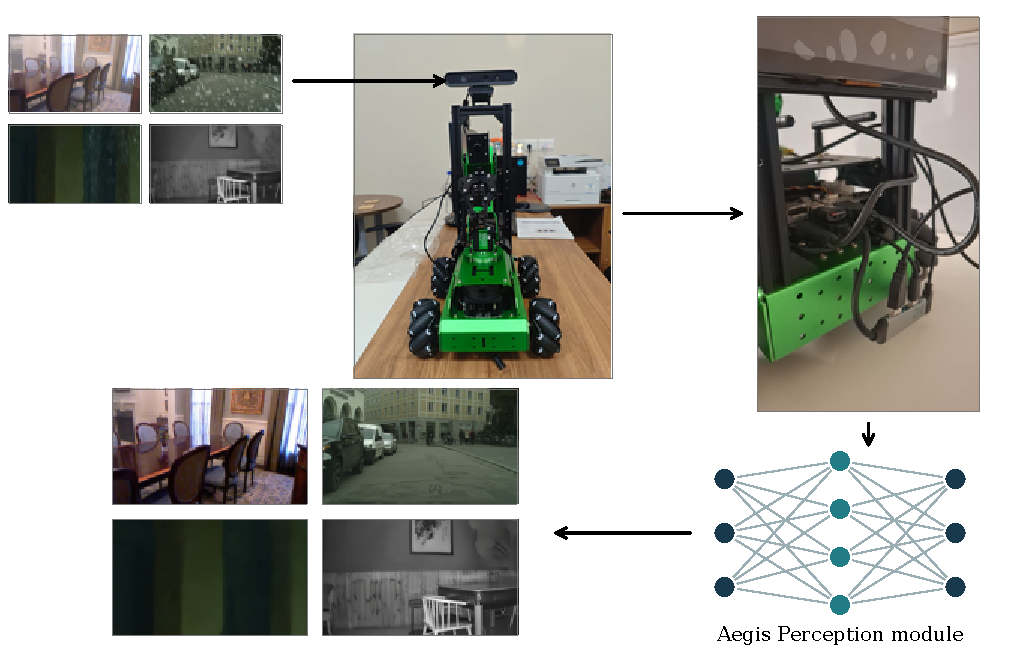
\includegraphics[width=\textwidth]{figures/cover_pipeline.pdf}
\vspace{5mm}
{\large
\begin{tabular}{@{}lr@{}}
Chitraksh & CS23B054\\[3mm]
Sudhanva & CS23B051\\[3mm]
Rishikesh & CS23B015
\end{tabular}\par}
\vspace{8mm}
{\large\textbf{Guide: Dr Vishnu Chalavadi}\par}
\vfill
{\large Indian Institute of Technology Tirupati\par}
\vspace{5mm}
{November 2026\par}
\vspace{3mm}
\end{titlepage}
\hypersetup{pageanchor=true}
\pagenumbering{roman}
\section*{Abstract}\addcontentsline{toc}{section}{Abstract}
Adverse-weather restoration must be judged by what it preserves for a vision
system as well as by its similarity to a clean image. This project studies
rain, fog, snow and smoke through three linked evaluations: a controlled
paired-image benchmark, fixed-detector comparisons, and execution on the
original 4\,GB Jetson Nano.

Six restoration systems are trained under a shared split and evaluation
protocol, with 18,610 training, 2,011 validation and 2,334 test pairs. Their
initialization sources differ. Restormer leads the balanced native-resolution
comparison at 32.58\,dB PSNR and 0.93 SSIM. Eight continuation arms test
spatial and detail adapters and auxiliary losses against matched further
training. No arm satisfies the validation replacement rule, so the original
epoch-51 checkpoint remains selected.

Downstream results depend on the complete processing path. In the earlier
72-image local DAWN pilot, pooled AP$_{50:95}$ rises from 29.97\% to 32.86\%,
with gains concentrated in fog. In the separately measured Nano cascade,
pooled AP falls from 29.59\% to 14.50\%. Labelled replay reaches only
0.61--0.62 frames/s with restoration, compared with 6.55--7.28 frames/s for
YOLO alone, while input energy increases to 11.35--11.59\,J/frame. Matched local
resolution controls demonstrate that both resampling and restoration can
change detections. An offline 8-bit weight grid fails two numerical-agreement
fixtures and retains FP32 storage and execution.

Six experimental phases are complete. The current exploratory phase investigates
RAMiT + YOLOv12 edge deployment, informed by the measured Restormer/YOLOv8n
limitations. The work establishes a reproducible comparison and identifies practical
failure modes. It does not establish universal detector improvement,
real-time edge operation, or an accepted INT8 acceleration. Single training
seeds, limited smoke backgrounds and short device trials bound the conclusions.

\textit{Keywords:} image restoration, adverse weather, Restormer, object
detection, controlled evaluation, Jetson Nano, quantization.
\begingroup
\setlength{\parskip}{0pt}
\tableofcontents
\endgroup
\clearpage

\pagenumbering{arabic}
\section{Project Overview}
\label{sec:outcomes}
Aegis Perception studies whether adverse-weather restoration improves both
image fidelity and object detection, and what that improvement costs on an
edge device. The experiments connect a four-weather benchmark to controlled
YOLOv8n comparisons and measurements on the original 4\,GB Jetson Nano.

\noindent\begin{minipage}{\linewidth}
\centering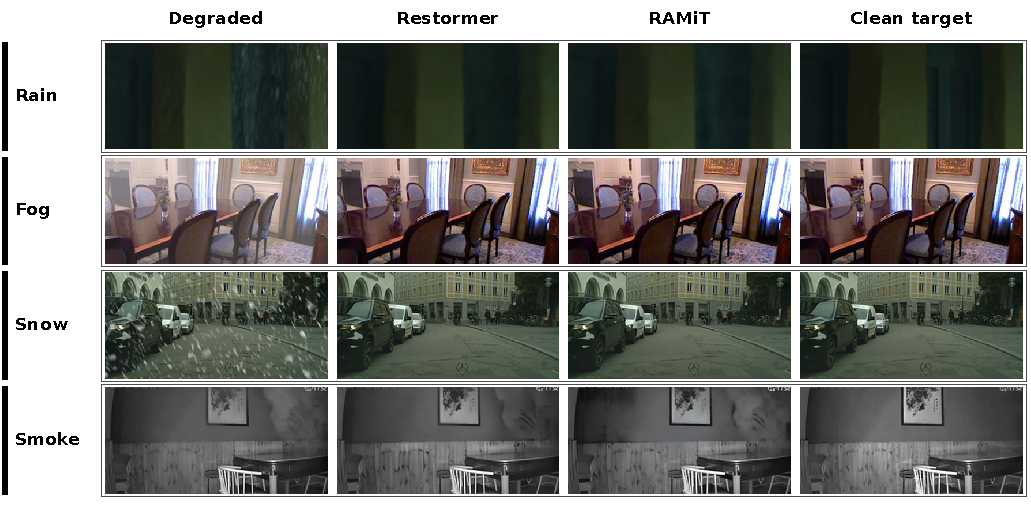
\includegraphics[width=\linewidth]{figures/weather_examples_mono.pdf}
\captionof{figure}{Four-weather restoration comparison. Each row shares one display crop; examples were fixed by sample-ID hash before score inspection. Saved predictions use native-resolution CPU FP32; the benchmark uses BF16.}
\label{fig:qual}
\end{minipage}

\medskip
\textbf{Reconstruction and detection.} Restormer leads the six-model benchmark,
but sharper-looking images do not guarantee better detection. The local pilot
improves AP; the smaller-canvas Nano cascade loses AP and throughput.

\medskip
\noindent\begin{minipage}{\linewidth}
\captionof{table}{Principal measurements. Compare raw and restored results within each experiment: the local pilot and Nano replay use different geometries and runtimes.}
\label{tab:opening-results}
\small\renewcommand{\arraystretch}{1.15}
\setlength{\fboxsep}{5pt}\setlength{\fboxrule}{.4pt}
\fbox{\begin{minipage}{\dimexpr\linewidth-2\fboxsep-2\fboxrule\relax}
\begin{tabularx}{\linewidth}{@{}p{.25\linewidth}Yp{.32\linewidth}@{}}\toprule
Experiment & Evaluation & Measured result\\\midrule
Restoration benchmark & Six models; 2,334 test pairs & Restormer: \textbf{32.58\,dB}; SSIM 0.93\\
Matched continuation & Eight ten-epoch arms & \textbf{Epoch 51 retained}\\
Local detection pilot & 72 images; $256\times448$ canvas & AP$_{50:95}$: 29.97\% $\rightarrow$ \textbf{32.86\%}\\
Nano detection & 72 images; $128\times128$ canvas & AP$_{50:95}$: 29.59\% $\rightarrow$ \textbf{14.50\%}\\
Nano labelled replay & YOLOv8n $\rightarrow$ Restormer + YOLOv8n & 6.55--7.28 $\rightarrow$ \textbf{0.61--0.62 FPS}\\
\bottomrule\end{tabularx}
\end{minipage}}
\end{minipage}

\smallskip
Six experimental phases are complete (Fig.~\ref{fig:timeline}). Their data, controls and
device measurements support the ongoing \textbf{RAMiT + YOLOv12 edge-deployment study};
end-to-end performance for this combination is not yet measured.
\clearpage

\section{Project Timeline and Contributions}
\label{sec:contributions}
The project was carried out by Chitraksh (CS23B054), Sudhanva (CS23B051) and
Rishikesh (CS23B015), under the guidance of Dr Vishnu Chalavadi.
Six experimental phases are complete. The current phase explores
RAMiT + YOLOv12 edge deployment.

\noindent\begin{minipage}{\linewidth}
\centering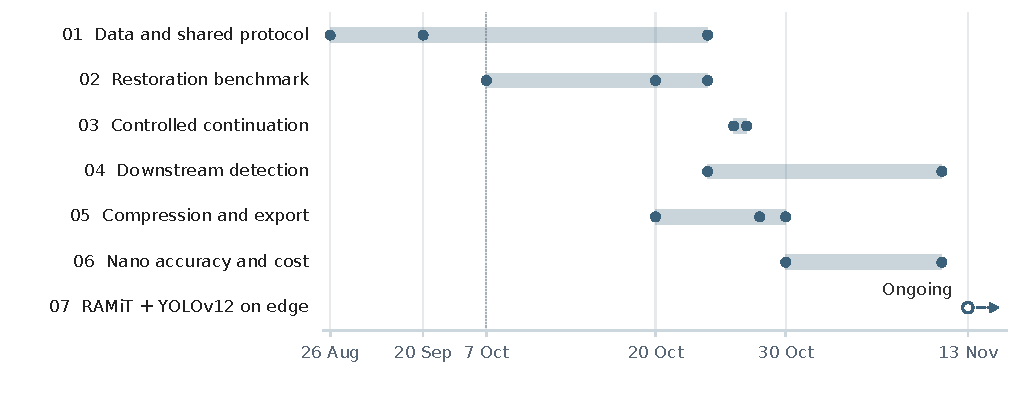
\includegraphics[width=\linewidth]{figures/work_timeline.pdf}
\captionof{figure}{Project timeline from dated records. Bars join the first and last milestones; dots identify records, not continuous daily effort. The axis is condensed before 7 October. Phase 7 is ongoing as of 13 November, with no completion date assigned.}
\label{fig:timeline}
\end{minipage}

\medskip
\noindent\begin{minipage}{\linewidth}
\captionof{table}{Individual and shared contributions to the six completed experimental phases. Entries identify recorded work; they do not assign exclusive ownership or percentages of effort.}
\label{tab:work-allocation}
\small\renewcommand{\arraystretch}{1.15}
\begin{tabularx}{\linewidth}{@{}p{.18\linewidth}YYY@{}}\toprule
Work package & Chitraksh & Sudhanva & Rishikesh\\\midrule
Data and protocol & Source/split review; metric interpretation & Split tooling; training configuration & Weather-level evaluation\\\addlinespace[3pt]
Six-model benchmark & Result review; benchmark context & Model implementation; training and selection & Cross-weather evaluation\\\addlinespace[3pt]
Continuation & Joint result review & Eight matched arms; validation selection & Joint result review\\\addlinespace[3pt]
Detection & Joint result review & Pilot tooling; resolution controls & Raw/resize/restored analysis\\\addlinespace[3pt]
Compression/export & Custom quantizer; pruning tooling & Trained export; adapter and checks & Compression/export evaluation\\\addlinespace[3pt]
Nano measurements & Joint result review & Nano runtime; export integration & Device-path analysis; FPS and power review\\\bottomrule
\end{tabularx}
\end{minipage}

\begin{multicols}{2}\raggedcolumns
\textbf{Research and compression.} Chitraksh's work connects source and
benchmark review to custom weight quantization and pruning. The integrated
edge handoff credits his quantizer; the 20 and 28 October commits record
these implementations. The tested weight grid was rejected by the numerical
screen.

\textbf{Models and integration.} Sudhanva configured and trained the models,
implemented the matched continuation experiments, and integrated the trained
exports and Nano runtime. Validation retained the original epoch-51 model.

\textbf{Evaluation.} Rishikesh's work covers restoration and detector
comparisons, export evaluation, and interpretation of Nano accuracy,
runtime and power. All three reviewed the experimental outputs and final
interpretation.

\textbf{Current work.} RAMiT + YOLOv12 integration and measured edge deployment
remain ongoing. No end-to-end accuracy or throughput result is yet claimed
for that combination.
\end{multicols}
\clearpage

\twocolumn[\noindent\begin{minipage}{\linewidth}
\centering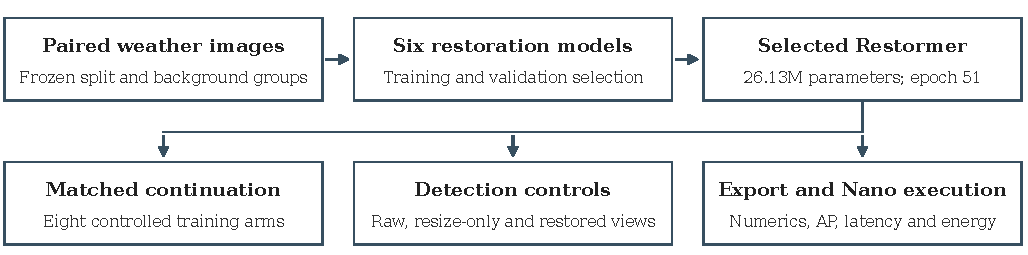
\includegraphics[width=\linewidth]{figures/project_evidence_flow.pdf}
\captionof{figure}{Experimental workflow. Epoch 51 initializes continuation and stays fixed for detection and Nano evaluation. Raw and resize-only views control the detector comparisons.}
\label{fig:project-workflow}
\end{minipage}

\vspace{10pt}
]
\section{Introduction}
\label{sec:introduction}
\subsection{Problem and motivation}
Rain, fog, snow and smoke obscure objects and reduce contrast. Restoration
can remove corruption, but it can also erase boundaries or lose detail during
resizing. Higher PSNR therefore need not improve detection.

Aegis Perception tests that distinction through paired-image benchmarks,
fixed-detector comparisons and execution on the original 4\,GB Jetson Nano.
The project follows one selected checkpoint from reconstruction to downstream
accuracy and processing cost (Fig.~\ref{fig:project-workflow}).

\subsection{Research questions and scope}
\begin{enumerate}
\item Which of six restoration recipes leads a shared four-weather benchmark?
\item Do model or loss changes outperform equal-budget continued training?
\item Does restoration help a fixed detector after controlling input geometry?
\item What accuracy, throughput and energy does the Nano cascade deliver?
\end{enumerate}
These questions produce six completed work packages (Fig.~\ref{fig:timeline}).
All models use reconstruction objectives; detector training and detector-loss
optimization lie outside the completed study. Different pretrained starting
points mean that the benchmark compares recorded recipes, not architecture alone.

\subsection{Main contribution}
The project connects an audited data split, six trained models, eight matched
continuation arms and measured detection/device results. The rejected
continuation changes and the Nano accuracy loss establish useful limits on
this pipeline. Supplementary Material preserves detailed controls, validation
trajectories and the evidence map.

\section{System Overview}
\label{sec:system}
\subsection{Experimental organization}
The training path and inference path have distinct roles.
Training receives paired degraded and target images and selects weights by
validation quality. Inference receives an adverse image, applies the selected
restorer, maps the result back to source geometry, and runs the same frozen
YOLOv8n detector used for the raw-input comparison. Figure~\ref{fig:project-workflow}
shows the common checkpoint linking the investigations.



\subsection{Problem formulation}
Let $x$ be an adverse-weather RGB image, $y$ its paired clean reference and
$f_\theta$ a restoration model. The reconstruction experiment measures
$\hat y=f_\theta(x)$ against $y$. Detection instead measures the predictions
of a fixed detector $g_\phi$ against object annotations $b$:
\begin{equation}
\hat b_{\rm raw}=g_\phi(T_D(x)),\qquad
\hat b_{\rm rest}=g_\phi(T_D(T_R^{-1}(f_\theta(T_R(x))))).
\end{equation}
Here $T_R$ is the restoration resize/pad operation and $T_R^{-1}$ denotes
cropping and mapping back to source geometry, not an invertible recovery of
lost pixels. $T_D$ is detector preprocessing. A resize-only control omits
$f_\theta$ while retaining the same $T_R$ and return mapping. This control is
necessary to distinguish restoration from the effects of geometry.

\begin{table*}[t]
\centering\small
\caption{What the project establishes at each evaluation stage.}
\label{tab:status}
\begin{tabularx}{\textwidth}{@{}p{.19\textwidth}YY@{}}
\toprule Stage & Recorded evidence & Boundary of the claim\\\midrule
Paired restoration & Six checkpoints; 14,004 model/image test rows & Native-resolution reconstruction; one training seed per model\\
Continuation & Eight ten-epoch arms; validation decisions & No accepted replacement of epoch 51\\
Local DAWN pilot & Raw, resize-only and restored views; 72 images & Fixed detector; specific $256\times448$ restoration canvas\\
Nano replay & 72 images, 541 objects; timing and power logs & Complete $128\times128$ cascade; one short run per condition\\
Resolution controls & 90 paths, three sources, five labelled objects & Diagnostic cases; camera predictions are unlabelled\\
Compression/export & Four-image weight/pruning screens and engine fixtures & Numerical acceptance is separate from task and device acceptance\\
\bottomrule
\end{tabularx}
\end{table*}

\subsection{Implementation organization}
The \texttt{src/aegis\_perception} package implements data loading, models,
training, inference and metrics. Separate scripts handle export, labelled
DAWN scoring and camera replay. Frozen configurations and saved outputs identify
executed experiments; Appendix~\ref{app:repro} maps them to the evidence.

\section{Related Work}
\label{sec:related}
\subsection{Restoration under multiple degradations}
Restormer~\cite{Zamir_2022_CVPR} uses transposed channel attention and gated
feed-forward layers for high-resolution restoration. Its channel-space
attention avoids constructing a full attention matrix over all image pixels.
This makes it a relevant quality baseline, while the convolutional projections
and intermediate features still impose a substantial execution cost.

TransWeather~\cite{Valanarasu_2022_CVPR} addresses different adverse-weather
corruptions within a transformer-based restoration model. PromptIR~\cite{NEURIPS2023_e187897e}
uses learned prompts to condition restoration on degradation information.
RAMiT~\cite{Choi_2024_CVPR} combines spatial and channel attention within a
lightweight restoration architecture. These methods motivate the comparison
of both quality and model size. Their original published results use different
datasets and training regimes; the results here belong to the project's
common fine-tuning and test protocol.

The project adds two implementation baselines: an attention-gated Pix2Pix
system and LiteWeather v2. The former combines an attention U-Net generator
and patch discriminator. The latter uses local residual blocks at high
resolution and attention with soft prompt conditioning at lower resolution.
Neither is presented as a reproduction of a separate published method with
the same name.

\subsection{Task utility and weather data}
Task-oriented restoration considers the downstream prediction objective,
rather than image fidelity alone~\cite{Chen_2025_CVPR,Gupta_2024_WACV}.
This motivates the fixed-detector experiments, but the completed Aegis models
are trained with reconstruction objectives. DAWN~\cite{Kenk_2020_DAWN}
provides real adverse-weather object annotations without paired clean targets.
It therefore answers a different question from the paired restoration benchmark.
RealRain-1k~\cite{Li_2022_RealRain} and SmokeBench~\cite{Jin_2025_SmokeBench}
also differ in scene type and reference acquisition; these distinctions
remain part of the interpretation of each weather score.

\subsection{Compression and efficient inference}
Integer-arithmetic quantization~\cite{Jacob_2018_CVPR} and hardware-aware
precision selection~\cite{Wang_2019_HAQ} connect representation choices to
an executable inference path. Transformer post-training quantization studies
address sensitivity and scale selection~\cite{Yuan_2022_PTQ4ViT,Li_2023_RepQ}.
A simulated weight grid is only an early check in that process: reconstructed
floating-point weights do not imply packed integer storage or integer kernels.

The NTIRE efficient super-resolution comparison reports runtime alongside
parameter count and quality~\cite{Ren_2025_CVPRW}. This distinction guides the
Aegis report: parameter count is a model property, while throughput depends
on resolution, operators, precision and the actual runtime. Focal frequency
loss~\cite{Jiang_2021_FFL} supplies an auxiliary objective for the controlled
continuation study; its inclusion is evaluated against the unchanged
architecture trained for the same additional budget.

\section{Datasets and Experimental Setup}
\label{sec:data}

\begin{figure}[!t]
\centering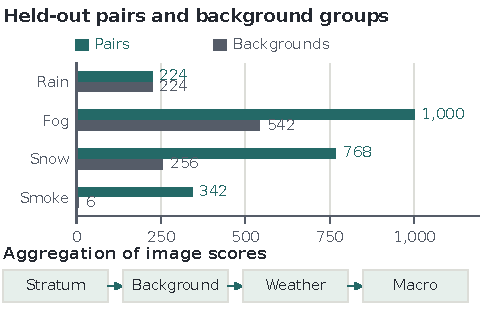
\includegraphics[width=\linewidth]{figures/benchmark_protocol.pdf}
\caption{Test coverage and aggregation. The 342 smoke pairs come from six backgrounds. Image scores are averaged within strata and then across strata, backgrounds, and weather conditions with equal weights at each level.}
\label{fig:benchmark-protocol}
\end{figure}

\begin{figure*}[t]
\centering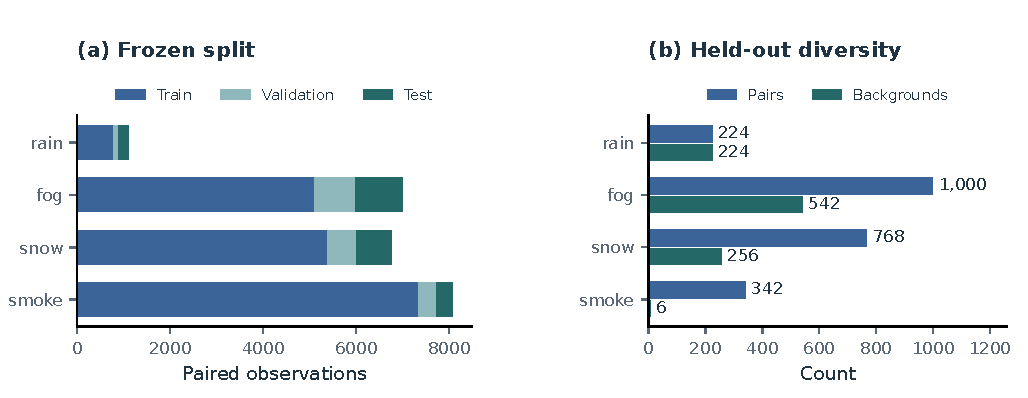
\includegraphics[width=\linewidth]{figures/dataset_coverage.pdf}
\caption{Completed data preparation: the frozen train/validation/test mixture and the distinction between held-out pairs and backgrounds. Smoke's many paired observations cover only six test backgrounds. Counts come from the saved split table.}
\label{fig:dataset-coverage}
\end{figure*}
\paragraph{Paired data.}
The active mixture combines processed real-rain pairs from RealRain-1k-H~\cite{Li_2022_RealRain}, synthetic haze from RESIDE-6K as a fog proxy, SnowCityscapes synthetic snow, and surveillance smoke from a repaired SmokeBench~\cite{Jin_2025_SmokeBench} partition. The source datasets supply all weather effects. Table~\ref{tab:data} and Fig.~\ref{fig:dataset-coverage} report the frozen split, including background groups. Figure~\ref{fig:benchmark-protocol} relates test coverage to the aggregation rule.

\begin{table}[!t]
\centering\small\setlength{\tabcolsep}{4pt}
\caption{Active paired split. Parentheses give background groups, which may contain related observations.}
\label{tab:data}
\begin{tabular}{@{}lrrr@{}}\toprule
Source & Train & Val. & Test\\\midrule
RealRain-1k-H &773 (755)&112 (112)&224 (224)\\
RESIDE-6K &5,102 (5,061)&897 (893)&1,000 (542)\\
SnowCityscapes &5,382 (1,794)&618 (206)&768 (256)\\
SmokeBench &7,353 (31)&384 (6)&342 (6)\\\midrule
Total pairs &18,610&2,011&2,334\\\bottomrule
\end{tabular}
\end{table}

A decode audit of 52,140 active and reserve files finds zero exact cross-split overlaps or near-target candidates under the specified thumbnail and pHash rule. The repaired split removes the identified smoke-reference overlap. Reserved snow/smoke pairs stay excluded from selection and testing. Sequence independence and alignment remain imperfectly characterized. Appendix~\ref{app:data} gives the audit thresholds and reserve counts.

\paragraph{Aggregation.}
For per-image RGB PSNR or SSIM $m_i$, let $I_s$ be images in stratum $s$, $S_g$ strata for background $g$, and $G_w$ backgrounds for weather $w$. We report
\begin{equation}
\bar m=\frac14\sum_w\frac1{|G_w|}\sum_{g\in G_w}
\frac1{|S_g|}\sum_{s\in S_g}\frac1{|I_s|}\sum_{i\in I_s}m_i.
\label{eq:metric}
\end{equation}
Strata rank thumbnail input/target differences within each background as a degradation proxy. Equal weighting at each level limits the influence of many variants from a single scene. Evaluation uses native-resolution BF16 forward passes and RGB in $[0,1]$, with MSE floor $10^{-12}$ and uniform $7\times7$ sample-covariance SSIM. Metrics precede 8-bit export. All 14,004 model/image rows support reaggregation. Cluster resampling estimates uncertainty conditional on these checkpoints and test groups.

\subsection{Training, validation and test responsibilities}
The sampler draws 4,096 pairs per epoch with replacement; this is not a pass
through all 18,610 training pairs. With global batch four, a 60-epoch run has
61,440 optimizer steps. Paired cropping and flipping preserve correspondence
between input and target. At evaluation, native images are padded as required
by the model and cropped back before scoring. The best validation macro PSNR
selects a checkpoint; the test partition supplies the reported comparison.

The 0.30/0.30/0.30/0.10 weather probabilities describe training draws.
They are independent of the equal-weather averaging used at evaluation.
Changing either sampling or aggregation changes the experimental question.
The fixed active manifest is therefore preserved rather than reconstructed
for this report.

\subsection{Metrics and uncertainty}
For $N$ RGB samples in $[0,1]$, the per-image peak signal-to-noise ratio is
\begin{equation}
\operatorname{PSNR}(y,\hat y)=10\log_{10}\!\left(\frac{1}{\max(\operatorname{MSE}(y,\hat y),10^{-12})}\right).
\end{equation}
The finite MSE floor prevents infinities in serialized outputs. SSIM uses
uniform $7\times7$ windows, sample covariance and the same unit data range.
The benchmark averages image-level scores hierarchically; it does not compute
PSNR from a pooled pixel MSE. Output comparisons for export use a separate
normalized tensor domain, described in Section~\ref{app:quant}.

The cluster bootstrap uses 2,000 resamples of the recorded test groups while
holding trained checkpoints fixed. It estimates conditional test uncertainty,
not variability across training seeds. There is one seed per system. The
six-model runs also use different pretrained starting weights, so the results
cannot isolate the causal effect of architecture from prior data exposure.

\subsection{Hardware and experimental domains}
Training uses BF16 on an NVIDIA A100-SXM4-40GB; the continuation study uses
two A100s with the same global batch. Native test inference uses BF16, while
the saved qualitative examples and local resolution diagnostics use CPU FP32.
The later on-device study uses the original 4\,GB Nano with L4T 32.7.3,
Python 3.6.9 and TensorRT 8.2.1.8. These domains are reported separately
because neither numerical agreement nor native-resolution quality can be
assumed to transfer unchanged across canvases and runtimes.

\section{Methodology and Implementation}
\label{sec:method}



\begin{figure*}[!t]
\centering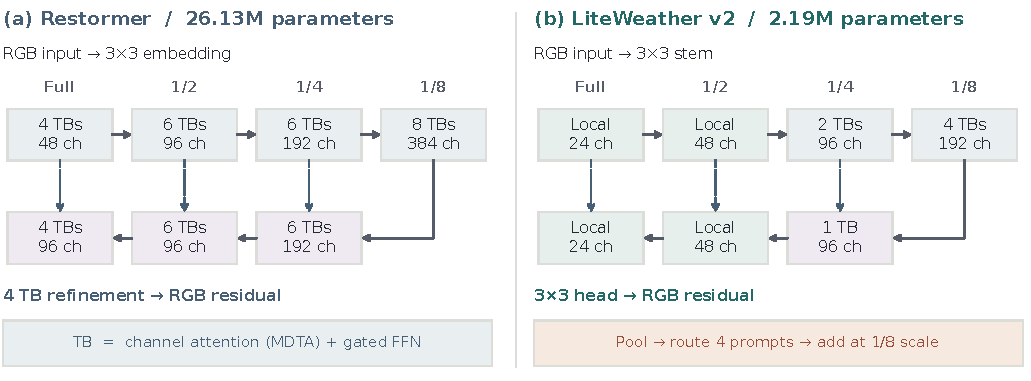
\includegraphics[width=\textwidth]{figures/restorer_architectures.pdf}
\caption{Architectures evaluated on the paired benchmark. Restormer uses transformer blocks (TBs) at all four scales. LiteWeather v2 uses local residual blocks at full and half resolution and attention at quarter and eighth resolution. Its soft prompt mixture is added before the eighth-scale transformer blocks. Arrows between scales represent down/up-sampling. Dashed arrows show encoder-to-decoder concatenation. Each network predicts a residual added to the degraded RGB image.}
\label{fig:architecture}
\end{figure*}

\paragraph{Shared training schedule.}
All six recipes use seed 42, 60 epochs, global batch four, and 4,096 paired draws per epoch with random $256\times256$ crops and flips. Background-aware sampling with replacement uses rain/fog/snow/smoke probabilities of 0.30/0.30/0.30/0.10. The non-GAN runs use L1 and AdamW, a $10^{-4}$ learning rate decayed to $10^{-6}$, $10^{-4}$ weight decay, and gradient clipping at 1.0. Attention Pix2Pix uses Adam, a patch discriminator, and adversarial loss plus $100$-weighted L1. BF16 training runs use an A100-SXM4-40GB. The best native-resolution validation macro PSNR selects the checkpoint.

\paragraph{Initialization and model identity.}
Attention Pix2Pix and LiteWeather v2 start from initialization. Restormer and RAMiT start from verified deraining weights, TransWeather from All-Weather weights, and PromptIR from its all-in-one weights. The published models use pinned sources and strict checkpoint loading. These recipes differ in prior data exposure.

\paragraph{Restormer.}
The epoch-51 model (26.13M parameters) connects the follow-up,
detection and export studies. Its encoder widths are $[48,96,192,384]$,
block counts $[4,6,6,8]$, and head counts $[1,2,4,8]$, with four refinement
blocks after decoding (Fig.~\ref{fig:architecture}a). All layers are fine-tuned;
selected weights are then frozen for evaluation and export~\cite{Zamir_2022_CVPR}.

\paragraph{Compact comparator.}
LiteWeather v2 (2.19M parameters) uses local residual blocks at full and
half resolution, two attention blocks at quarter scale and four at eighth
scale, with four and eight heads respectively (Fig.~\ref{fig:architecture}b).
A learned prompt mixture conditions its latent features without weather labels.

\subsection{Attention and residual reconstruction}
The implemented Restormer forms query, key and value tensors with a
$1\times1$ convolution followed by a depthwise $3\times3$ convolution.
Within each head, $Q$ and $K$ are normalized along the spatial dimension.
With $c_h$ channels per head and $n$ spatial positions, they have shape
$c_h\times n$. The implemented attention is
\begin{equation}
 A=\softmax(\tau\,\bar Q\bar K^\top),\qquad
 Z=W_o(AV),
\end{equation}
where $A$ has shape $c_h\times c_h$ and $\tau$ is a learned temperature.
Layer normalization and residual connections surround attention and the
feed-forward sublayer. That sublayer splits depthwise-filtered projected
features into $U$ and $V$, gates them as $\operatorname{GELU}(U)\odot V$,
and projects back to the block width. The decoder uses upsampling and skip
concatenation, followed by refinement and an RGB residual added to the input.
These are the existing Restormer mechanisms.

LiteWeather v2 conditions its latent representation $F$ using four learned
prompt vectors $p_j$:
\begin{equation}
 \alpha=\softmax(W_r\GAP(F)+b_r),\qquad
 F'=F+\sum_{j=1}^{4}\alpha_jp_j.
\end{equation}
The router receives image features rather than ground-truth weather labels.
The evaluated checkpoint uses widths $[24,48,96,192]$. The preserved earlier
convolution-only LiteWeather module is a different model.

\subsection{Model loading and identity}
Pinned upstream implementations use strict state loading: shape or key
mismatches are rejected. The selected Restormer inference package retains
26,126,644 parameters in 104,701,712 bytes. Continuation, downstream and export
studies use this same checkpoint; the historical rain-only checkpoint is
separate. The shared comparison evaluates complete training recipes, including
the differing initialization sources and objectives described above.

\subsection{Controlled adapter design}
The experimental context/detail adapter is inserted after the latent and
third-level decoder stages while preserving backbone parameter names.
It normalizes and reduces features to width 64. A $5\times5$ average filter
forms a low-frequency estimate, and subtracting it forms a local high-pass
component. A sigmoid gate receives mean absolute low/high feature magnitudes.
The spatial branch pools to an $8\times8$ token grid and applies four-head
spatial attention; the detail branch filters the high-pass component with
a depthwise $5\times5$ kernel and GELU.

Zero-initialized output projections preserve the starting backbone.
Spatial-attention logits and softmax remain FP32 under mixed precision.
This enables matched spatial-only, detail-only and combined arms. Average
filtering is an implementation choice, not a physical separation of weather
and scene content (Section~\ref{sec:jointresults}).

\clearpage\onecolumn
\section{Restoration Results}
\label{sec:restoration-results}

\noindent\begin{minipage}{\linewidth}
\centering\comparisonplot[\textwidth]{figures/benchmark_tradeoffs.pdf}
\captionof{figure}{Performance across six trained systems. \textbf{(a)} Macro PSNR versus parameter count. Bars are 95\% cluster-bootstrap intervals conditional on the fixed checkpoints and test groups. The dashed segment connects the measured quality--size frontier. \textbf{(b)} Weather-balanced PSNR gain over the degraded input. Smoke has the smallest gains for all six systems.}
\label{fig:size}
\end{minipage}
\medskip
\noindent\begin{minipage}{\linewidth}
\centering\comparisonplot[.94\linewidth]{figures/weather_psnr.pdf}
\captionof{figure}{The completed six-model benchmark as a weather-by-model comparison. Restormer leads rain, snow and smoke; PromptIR leads fog. Each cell is the recorded balanced test PSNR, rounded to two decimals. The underlying comparison uses full precision.}
\label{fig:weather-psnr}
\end{minipage}
\medskip
\noindent\begin{minipage}{\linewidth}
\centering\small\setlength{\tabcolsep}{4pt}
\captionof{table}{Native-resolution test results on 2,334 pairs. Weather columns report PSNR in dB. SSIM is scaled by 100 for display. Macro metrics follow Eq.~\ref{eq:metric}. Bold marks the best measured values.}
\label{tab:six}
\begin{tabular}{@{}lrrrrrrrr@{}}\toprule
Model & Params (M)& Epoch & Rain & Fog & Snow & Smoke & Macro PSNR & SSIM $\times100$\\\midrule
Restormer & 26.13 & 51 & \textbf{38.77} & 31.51 & \textbf{39.51} & \textbf{20.55} & \textbf{32.58} & \textbf{92.97}\\
PromptIR & 35.59 & 50 & 36.40 & \textbf{31.88} & 37.63 & 19.65 & 31.39 & 91.82\\
TransWeather & 38.05 & 58 & 34.19 & 29.58 & 32.31 & 20.10 & 29.04 & 90.00\\
RAMiT & \textbf{0.93} & 45 & 34.37 & 24.19 & 36.85 & 19.23 & 28.66 & 89.95\\
LiteWeather v2 & 2.19 & 59 & 31.02 & 27.42 & 31.40 & 18.98 & 27.21 & 86.44\\
Attention Pix2Pix & 29.85 & 59 & 28.46 & 23.55 & 29.05 & 17.85 & 24.73 & 82.01\\\bottomrule
\end{tabular}
\end{minipage}
\begin{multicols}{2}\raggedcolumns
\paragraph{Quality and model size.}
The weather-wise comparison in Fig.~\ref{fig:weather-psnr} makes the model trade-offs explicit. Restormer gains 13.97 dB over degraded inputs and leads three of four weather columns (Tab.~\ref{tab:six}). PromptIR leads fog PSNR by 0.38 dB. RAMiT uses about $28\times$ fewer parameters than Restormer, with a 3.92 dB macro gap (Fig.~\ref{fig:size}a). LiteWeather v2 closes part of the fog gap relative to RAMiT, but trails it on macro PSNR. The device trials in Sec.~\ref{sec:edge} address execution.

\paragraph{Smoke is the clearest remaining weakness.}
Restormer's smoke gain is 2.34 dB, versus 15.92--21.11 dB on the other weathers (Fig.~\ref{fig:size}b). Of 342 smoke images, 27 lose PSNR and 37 lose SSIM relative to the raw input. Attention Pix2Pix also regresses on balanced smoke PSNR and SSIM. The qualitative panels (Fig.~\ref{fig:qual}) show streak and snow removal, increased contrast in haze, and residual smoke compared with the target. Six smoke backgrounds limit generalization from these outcomes.
\end{multicols}
\clearpage
\noindent\begin{minipage}{\linewidth}
\centering
\comparisonplot[\textwidth]{figures/restoration_gain_histograms.pdf}
\captionof{figure}{Distributions of per-image PSNR improvement over degraded input for Restormer and RAMiT, using the same 2,334 held-out paired images per model. Histograms use 2 dB bins and normalize each model within each weather to 100\%. Each image has equal weight here; these descriptive distributions are distinct from the group- and weather-balanced benchmark means. Restormer's median gain is higher in all four weather groups; smoke retains a negative-gain tail.}
\label{fig:restoration-gain-histograms}
\end{minipage}
\begin{multicols}{2}\raggedcolumns
\paragraph{Distribution of improvement.}
Figure~\ref{fig:restoration-gain-histograms} adds the per-image view to the
balanced means. Restormer's median gain exceeds RAMiT's in all four weather
groups, while the smoke distribution includes degraded examples that lose
PSNR. These distributions describe reconstruction; the ongoing RAMiT--YOLOv12
phase still requires an integrated detector and device evaluation.
\end{multicols}

\section{Continuation with Matched Training}
\label{sec:jointresults}
\subsection{Design and replacement rule}
\label{sec:jointmethod}
\begin{multicols}{2}\raggedcolumns
All eight arms start from epoch 51 and continue for ten epochs with seed 42,
global batch four on two A100s, and 4,096 weighted draws per epoch
(10,240 updates per run). They use paired $256\times256$ crops, BF16,
AdamW with $\beta=(0.9,0.999)$, weight decay $10^{-4}$, gradient clipping 1.0,
and learning rate $2\times10^{-5}$ decayed to $10^{-6}$.

The control retains the original architecture and L1 loss. Zero-start spatial
and detail adapters use width 64, four heads and grid eight. The recipe-only
arm keeps the network unchanged; combined-adapter arms test SSIM, focal
frequency loss (FFL), and both auxiliaries:
\begin{equation}
\mathcal L=\mathcal L_1+\lambda_S\mathcal L_{\rm SSIM}
+\lambda_F\mathcal L_{\rm FFL}.
\end{equation}
Auxiliary weights use full-network FP32 gradient norms from 64 paired
training crops:
\begin{equation}
\lambda_a=0.1\operatorname{median}_i\left(
\frac{\|\nabla_\theta\mathcal L_{1,i}\|_2}{\|\nabla_\theta\mathcal L_{a,i}\|_2}\right).
\end{equation}
This gives $\lambda_S\approx7.81\times10^{-2}$ and $\lambda_F\approx3.10$;
exact values remain in the saved configuration and are fixed before
continuation~\cite{Jiang_2021_FFL}.

Raw and EMA states (decay 0.999) compete by validation macro PSNR. Replacement
requires at least 0.10\,dB over both initialization and matched control,
retained macro SSIM, and per-weather losses no greater than 0.10\,dB and
0.001 SSIM. All eight arms fail this rule; the epoch-51 model is retained
before test evaluation.
\end{multicols}
\clearpage
\noindent\begin{minipage}{\linewidth}
\centering\comparisonplot[\linewidth]{figures/continuation_millidb.pdf}
\captionof{figure}{Completed continuation experiments relative to the matched further-training control. Milli-decibels keep the small differences readable with two decimal places. The control improves over the original checkpoint by 118.97 mdB, while the best additional gain is 28.81 mdB. No arm passes the validation replacement rule.}
\label{fig:joint}
\end{minipage}
\medskip
\noindent\begin{minipage}{\linewidth}
\centering\comparisonplot[\textwidth]{figures/continuation_validation_gate.pdf}
\captionof{figure}{Validation replacement criterion for the eight continuation arms. Panels compare selected checkpoints with the epoch-51 starting checkpoint and matched continuation control. Both improvements must reach the dashed $+0.10$ dB threshold before applying SSIM and per-weather retention criteria.}
\label{fig:continuation-gate}
\end{minipage}
\medskip
\noindent\begin{minipage}{\linewidth}
\centering\small\setlength{\tabcolsep}{4pt}
\captionof{table}{Recorded follow-up validation checkpoints. All selected states are EMA; all eight replacements fail. Parameters include added adapters.}
\label{tab:jointval}
\begin{tabular}{@{}lrrrr@{}}\toprule
Arm & Params (M)& Epoch & PSNR & SSIM $\times100$\\\midrule
Continuation control &26.13&6&32.49&92.11\\
Spatial &26.23&6&32.49&92.11\\
Detail &26.20&6&32.49&92.11\\
Combined &26.27&6&32.49&92.11\\
Recipe only &26.13&6&32.49&92.17\\
Combined + SSIM &26.27&6&32.51&92.19\\
Combined + FFL &26.27&6&32.47&92.08\\
Combined + recipe &26.27&5&32.49&92.16\\
\bottomrule\end{tabular}
\end{minipage}

\begin{multicols}{2}\raggedcolumns
\textbf{Validation decision.} Seven arms select EMA at epoch six; combined
+ recipe selects EMA at epoch five (Table~\ref{tab:jointval}). The largest
validation gain over control is 17.96\,mdB, below the 0.10\,dB replacement
threshold (Fig.~\ref{fig:continuation-gate}).

\textbf{Held-out comparison.} The control reaches 32.70\,dB, a gain of
118.97\,mdB over epoch 51. Adapters add only 1.50--5.88\,mdB beyond matched
training. The unchanged-network loss recipe gives the largest additional
PSNR gain, 28.81\,mdB; combined + SSIM gives the highest scaled SSIM, 93.17.
Table~\ref{tab:jointweather} retains the weather breakdown. These small
single-seed differences do not justify replacing the selected model.
\end{multicols}
\clearpage

\section{Detection Across Operating Points}
\label{sec:dawn}

\noindent\begin{minipage}{\linewidth}
\centering\comparisonplot[\textwidth]{figures/dawn_operating_points_spaced.pdf}
\captionof{figure}{Labelled DAWN detection in the earlier local pilot and the Nano benchmark. The local comparison includes a $256\times448$ resize-only view. The Nano comparison evaluates the complete cascade with a $128\times128$ Restormer canvas. Both use 72 images, 24 per weather. Signed values show restored-minus-raw AP in percentage points within each evaluation.}
\label{fig:det}
\end{minipage}
\medskip
\noindent\begin{minipage}{\linewidth}
\centering\comparisonplot[\textwidth]{figures/controlled_resolution.pdf}
\captionof{figure}{Matched local resolution diagnostic. \textbf{(a)} The same degraded source enters all branches. Native restoration only pads and crops. Each branch maps to the source geometry and uses the same detector preprocessing. \textbf{(b)} Correct detections among two annotated vehicles in one DAWN scene. Under rain, the 256 resize-only view already recovers both vehicles. Native restoration gains a match in rain and loses one in smoke.}
\label{fig:resolution}
\end{minipage}
\begin{multicols}{2}\raggedcolumns
\paragraph{Earlier local pilot.}
DAWN~\cite{Kenk_2020_DAWN} supplies real-weather road-object labels. The earlier local evaluation compares raw, resize-only, and restored views on 72 labelled images with one frozen COCO-pretrained YOLOv8n. The two transformed views use a $256\times448$ canvas and return to original geometry before $640\times640$ detector preprocessing. Pooled AP$_{50:95}$ rises from 29.97\% raw to 32.86\% restored, with the resize-only control at 29.25\%. Fog improves by 10.12 points against raw input. Rain and snow decline by 1.66 and 0.65 points (Fig.~\ref{fig:det}a).

\paragraph{Labelled Nano benchmark.}
The measured Nano evaluation has 72 images and 541 labelled objects across fog, rain, and snow. The $128\times128$ Restormer path returns to source geometry before the fixed FP32 YOLOv8n engine shared by the two Nano arms. Pooled AP$_{50:95}$ falls from 29.59\% to 14.50\%, a 15.08-point loss (Fig.~\ref{fig:det}b). At confidence 0.25 and IoU 0.50, matched objects fall from 270 to 110, and misses rise from 271 to 431. AP uses detections from confidence 0.001, class-aware NMS at 0.7, and at most 100 detections per image. Geometry, runtime, and scoring differ from the earlier local pilot. The measured drop pertains to the complete Nano cascade.


\end{multicols}

\clearpage\onecolumn
\subsection{128-pixel canvas: matched people comparisons}
\noindent\begin{minipage}{\linewidth}
\centering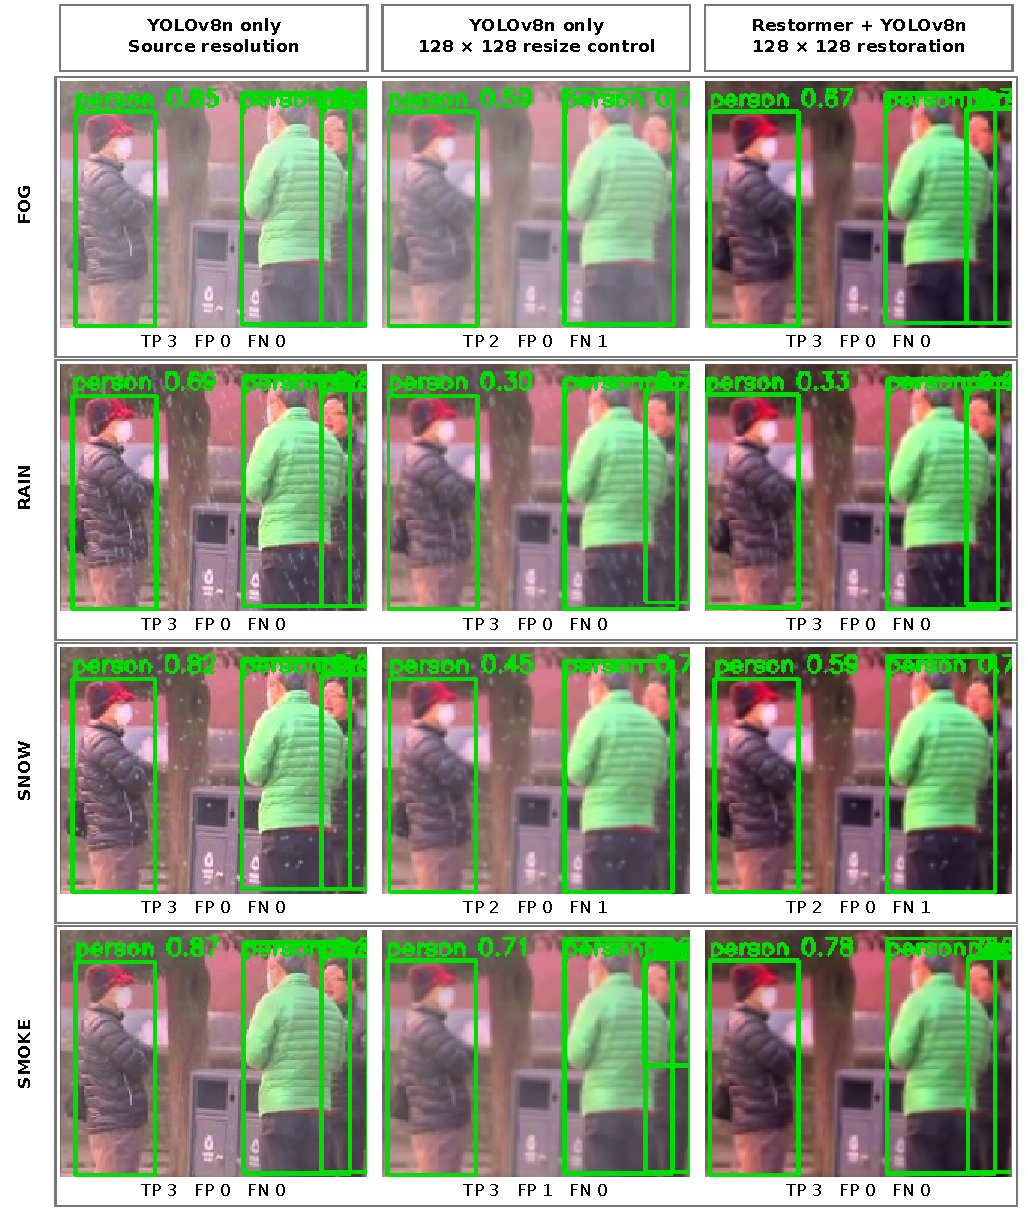
\includegraphics[width=\linewidth]{figures/matched_128_people.pdf}
\captionof{figure}{The same three labelled people under four added-weather conditions, using the identical pipeline and thresholds as Figure~\ref{fig:matched-128-vehicles}. Full saved overlays are shown. Relative to the 128 resize control, Restormer recovers one person in fog and removes an unmatched prediction in smoke; one person remains missed in snow. All three are found in rain. These are repeated views of one source scene, not independent benchmark images. Original sources already contain haze.}
\label{fig:matched-128-people}
\end{minipage}

\clearpage\twocolumn
\renewcommand{\dbltopfraction}{.85}
\renewcommand{\topfraction}{.85}
\section{Edge Execution and Compression}
\label{sec:edge}

\begin{figure}[!t]
\centering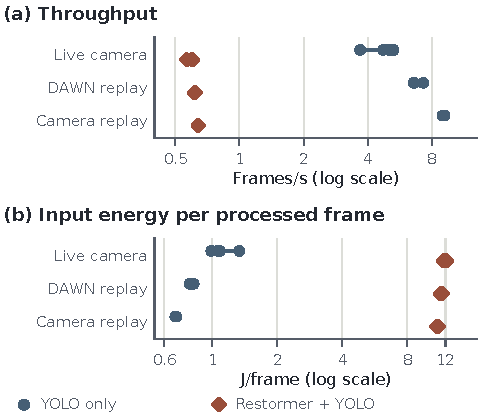
\includegraphics[width=\linewidth]{figures/nano_runtime.pdf}
\caption{Original Jetson Nano throughput and board input energy. Each point is one weather condition. The lines span conditions within a workload. Live application FPS and replay FPS have different timing boundaries. Energy uses integrated board input power divided by processed frames.}
\label{fig:nano-runtime}
\end{figure}

\paragraph{Measured Nano execution.}
Figure~\ref{fig:nano-runtime} separates live, labelled replay, and saved-camera replay. In DAWN replay, YOLO alone reaches 6.55--7.28 FPS with median pipeline latency of 129.2--147.2\,ms. Adding the $128\times128$ restorer yields 0.61--0.62 FPS and 1,596.7--1,619.6\,ms. Board input energy rises from 0.78--0.82 to 11.35--11.59\,J/frame, about 14--15 times more across weather subsets. The live cascade runs at 0.57--0.60 FPS. Live throughput includes capture, weather generation, display, and application overhead. Replay isolates the processing path. Power integrates the board input rail without subtracting idle power. Short, single-run windows constrain runtime and energy estimates (Appendix~\ref{app:hardware}).

\begin{figure*}[t]
\centering
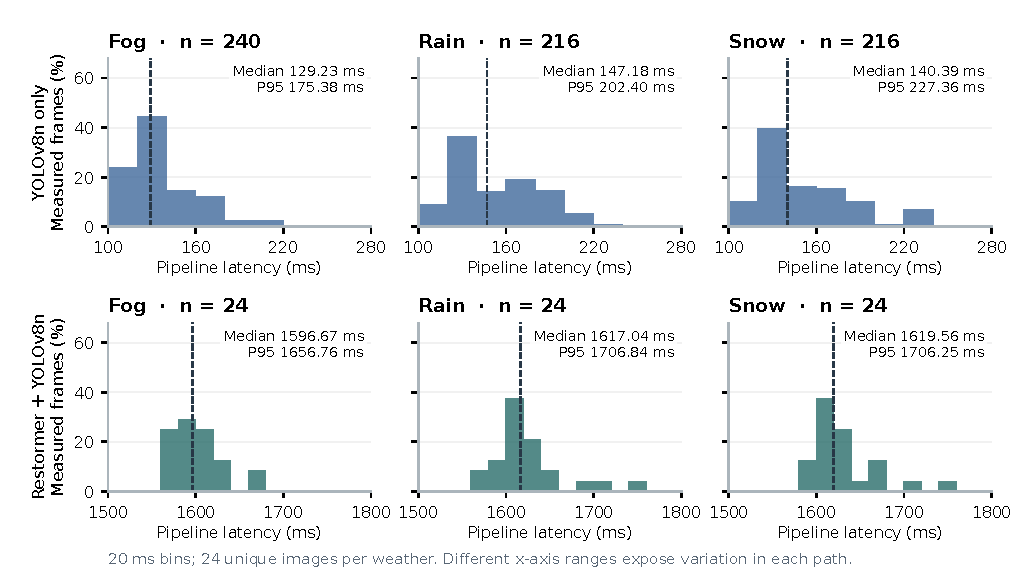
\includegraphics[width=.98\textwidth]{figures/nano_pipeline_latency_histograms.pdf}
\caption{Measured per-frame pipeline latency on the Jetson Nano for YOLOv8n alone and Restormer ($128\!\times\!128$ restoration canvas) followed by YOLOv8n. The saved labelled replay uses 24 unique images per weather and five excluded warm-up frames. The raw path repeats the images to record 240/216/216 timed frames; the restored path records 24 per weather, with each window lasting at least 30 seconds. Histograms use 20 ms bins and normalize each run to 100\%; dashed lines mark medians. The two rows deliberately use different latency ranges. Timing covers synchronized restoration/resize and detector preprocessing, inference and NMS; capture, decoding, weather synthesis, scoring and preview are excluded.}
\label{fig:nano-latency-histograms}
\end{figure*}


Figure~\ref{fig:nano-latency-histograms} shows the full measured latency
distributions. Median raw pipeline latency is 129.23--147.18\,ms, compared
with 1,596.67--1,619.56\,ms after adding Restormer. The observations repeat
images within the recorded runs; they are not independent repeated trials
or live-camera timing.

\paragraph{Conversion and deployment.}
The measured cascade uses FP32 YOLOv8n and a mixed FP16/FP32 Restormer on the original 4\,GB Jetson Nano with TensorRT 8.2.1.8. Its detector and restorer pass three and four numerical fixtures, respectively. Lower-precision weights can reduce storage and memory traffic when the runtime packs and executes them. The separate 8-bit weight grid retains FP32 execution and storage at 105,748,439 bytes. Fog and smoke exceed its output RMSE limit at $6.18\times10^{-3}$ and $4.64\times10^{-3}$. The 8-bit candidate and pruning controls remain offline screens (Section~\ref{app:quant}).

\subsection{Memory observations}
\begin{figure*}[t]
\centering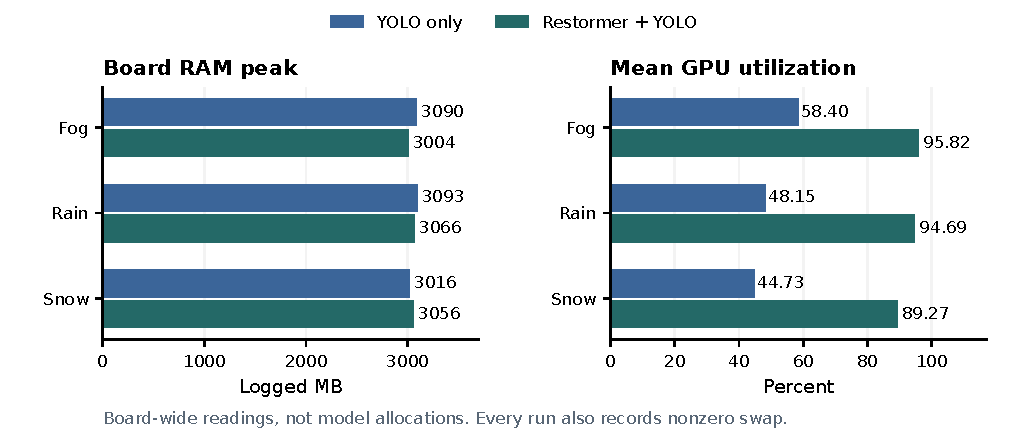
\includegraphics[width=.98\linewidth]{figures/nano_resources.pdf}
\caption{Resource observations from the completed Nano replay. The cascade uses the GPU more heavily, while board-wide RAM peaks remain near 3 GB. These logged peaks include other board processes and do not measure the restorer's isolated allocation.}
\label{fig:nano-resources}
\end{figure*}
\begin{table}[t]
\centering\small
\caption{Recorded board memory and GPU utilization during labelled DAWN replay. RAM and swap are board-wide peaks in the logged MB units, not isolated model allocations.}
\label{tab:memory}
\begin{tabular}{@{}llrrr@{}}\toprule
Weather & Path & RAM & Swap & GPU (\%)\\\midrule
Fog & YOLO & 3090 & 1384 & 58.4\\
Fog & Cascade & 3004 & 1368 & 95.8\\
Rain & YOLO & 3093 & 1384 & 48.1\\
Rain & Cascade & 3066 & 1378 & 94.7\\
Snow & YOLO & 3016 & 1384 & 44.7\\
Snow & Cascade & 3056 & 1382 & 89.3\\
\bottomrule
\end{tabular}
\end{table}

Figure~\ref{fig:nano-resources} and Table~\ref{tab:memory} supplement timing with the recorded memory context.
All six labelled replay runs report nonzero swap. Mean GPU utilization is
89.3--95.8\% for the cascade and 44.7--58.4\% for YOLO alone. These are
whole-board observations from the short workloads; they do not isolate the
restorer's allocation or prove that swap caused the latency difference.

\subsection{Weight Discretization and Pruning}
\label{app:quant}
\subsubsection{Weight-grid transformation}

The ONNX adapter identifies convolution initializers from graph edges. It preserves two boundary tensors and discretizes 272 convolution tensors, including attention projections and feed-forward convolutions. Activations, matrix attention, normalization, storage, and runtime remain FP32 (Fig.~\ref{fig:weight-grid}).

For each output channel of $m$ weights, the order statistic is $k=\max(1,\operatorname{round}(0.9995m))$. With $a$ the $k$th absolute weight magnitude, the scale is $s=\max(a,10^{-8})/127$. The zero point is zero, and PyTorch rounding gives
\begin{equation}
q=\clip(\operatorname{round}(w/s),-128,127),\qquad \tilde w=sq.
\end{equation}
Small kernels may select their maximum magnitude. The reconstructed $\tilde w$ replaces the FP32 initializer. Both serialized ONNX graphs occupy 105,748,439 bytes.

\subsubsection{Quality retention and output agreement}
For the normalized $[-1,1]$ output tensors $z$ and $\tilde z$, agreement uses
\begin{equation}
e_{\rm rms}=\sqrt{\tfrac1N\sum_j(\tilde z_j-z_j)^2},
\quad e_{\infty}=\max_j|\tilde z_j-z_j|.
\end{equation}
Quality is evaluated on cropped RGB $[0,1]$ against the clean target. RGB PSNR uses a $10^{-12}$ MSE floor. SSIM uses a uniform $7\times7$ window, sample covariance, and constants $0.01^2$ and $0.03^2$. The four-fixture gate requires $\Delta\mathrm{PSNR}\geq-0.1$ dB, $\Delta\mathrm{SSIM}\geq-0.001$, $e_{\rm rms}\leq0.004$, and $e_\infty\leq0.05$, with finite outputs and matching shapes. Fog and smoke fail the RMSE condition.

\FloatBarrier
\begin{figure*}[!t]
\centering\resizebox{\textwidth}{!}{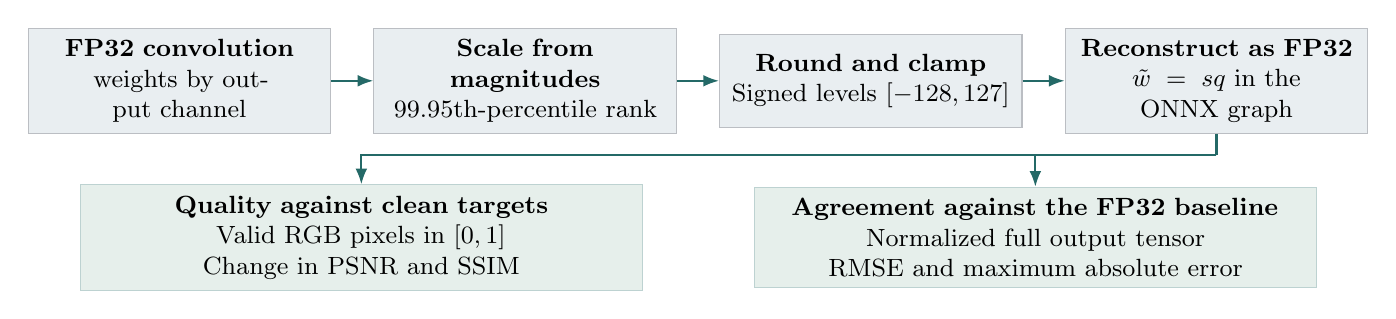
\begin{tikzpicture}[
  x=1cm,y=1cm,
  op/.style={draw=aegisgray!40,fill=aegishead,text width=3.56cm,
    minimum height=1.18cm,inner sep=4pt,align=center,font=\small},
  check/.style={draw=aegisblue!30,fill=aegisbest,text width=6.85cm,
    minimum height=1.08cm,inner sep=4pt,align=center,font=\small},
  flow/.style={-{Latex[length=2.0mm]},aegisblue,line width=.76pt}]
\node[op] (weights) at (1.96,0) {\textbf{FP32 convolution}\\weights by output channel};
\node[op] (scale) at (6.35,0) {\textbf{Scale from magnitudes}\\99.95th-percentile rank};
\node[op] (grid) at (10.74,0) {\textbf{Round and clamp}\\Signed levels $[-128,127]$};
\node[op] (onnx) at (15.13,0) {\textbf{Reconstruct as FP32}\\$\tilde w=sq$ in the ONNX graph};
\draw[flow] (weights) -- (scale);
\draw[flow] (scale) -- (grid);
\draw[flow] (grid) -- (onnx);
\node[check] (reference) at (4.27,-1.99) {\textbf{Quality against clean targets}\\Valid RGB pixels in $[0,1]$\\Change in PSNR and SSIM};
\node[check] (output) at (12.83,-1.99) {\textbf{Agreement against the FP32 baseline}\\Normalized full output tensor\\RMSE and maximum absolute error};
\coordinate (branch) at (15.13,-.94);
\draw[aegisblue,line width=.76pt] (onnx.south) -- (branch);
\draw[flow] (branch) -| (reference.north);
\draw[flow] (branch) -| (output.north);
\end{tikzpicture}
}
\caption{Weight-grid screen. Convolution weights are discretized per output channel and reconstructed in FP32. Clean-target quality uses cropped valid RGB pixels. Numerical agreement uses the full normalized output tensor.}
\label{fig:weight-grid}
\end{figure*}

\begin{table}[!t]
\centering\small
\caption{Absolute clean-reference quality and maximum output error for the 8-bit weight grid. SSIM and output error are scaled by 100 for display.}
\begin{tabular}{@{}lrrrr@{}}\toprule
Weather & Base PSNR & Grid PSNR & SSIM $\times100$ & $100e_\infty$\\\midrule
Rain &34.28&34.37&95.82&2.45\\
Fog &24.36&24.38&88.93&4.67\\
Snow &36.96&36.89&97.39&2.54\\
Smoke &21.84&21.87&83.96&2.14\\\bottomrule
\end{tabular}
\end{table}

\begin{figure*}[!t]
\centering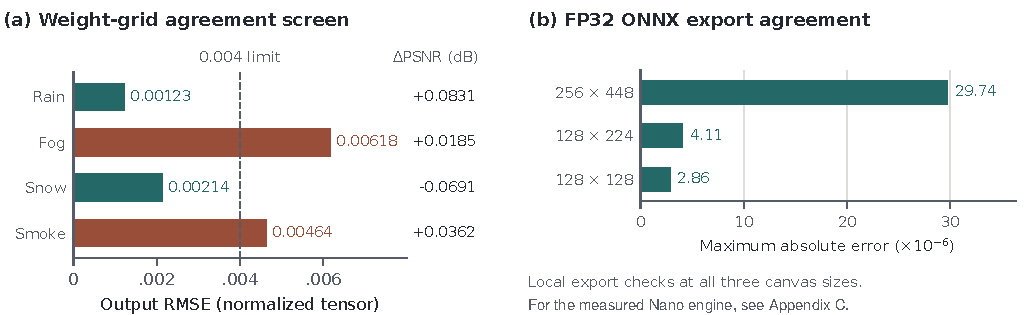
\includegraphics[width=\textwidth]{figures/edge_acceptance_current.pdf}
\caption{Offline numerical screens. \textbf{(a)} Weight-grid RMSE on normalized outputs, alongside clean-target PSNR changes. Fog and smoke exceed the 0.004 gate. \textbf{(b)} Local FP32 PyTorch--ONNX agreement by canvas size. Earlier build observations describe the path to the separately evaluated mixed engine in Appendix~\ref{app:hardware}.}
\label{fig:edge}
\end{figure*}

\subsubsection{Linear-only conversion and pruning controls}
A dynamic conversion restricted to linear modules finds no eligible layers. It converts zero modules and preserves all state tensors. Restormer uses convolutions for its projection layers.

\begin{figure}[!t]
\centering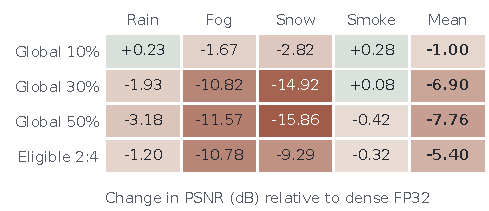
\includegraphics[width=\linewidth]{figures/pruning_screen_matrix.pdf}
\caption{Pruning changes in PSNR on four fixtures. The mean weights fixtures equally. Every masked variant fails the retention screen.}
\label{fig:pruning-screen}
\end{figure}
Global magnitude pruning masks convolution weights without retraining. The eligible 2:4 mask produces 39.68\% sparsity over the tested population of 26,096,544 convolution weights. All masked state dictionaries remain 104,696,534 bytes, with explicit zeros in dense tensors. Figure~\ref{fig:pruning-screen} shows the per-fixture quality losses. At 10\% global sparsity, fog and snow fail both quality criteria, and smoke fails its SSIM criterion.


\section{Lessons and Ongoing Deployment}
\label{sec:discussion}

\subsection{What the measurements establish}
\textbf{Reconstruction.} Restormer leads the six-model benchmark; RAMiT is
smaller but has no matched cascade/device measurements. All continuation
variants fail validation replacement, so epoch 51 remains selected.

\textbf{Detection and cost.} Local AP improves; Nano AP and throughput decline.
Different canvases, runtimes and scoring prevent attributing the gap to
resolution or precision alone. The five-object geometry diagnostic cannot
replace a full labelled resize-only Nano arm. Camera fidelity scores and
illustrative overlays do not establish object accuracy.

\subsection{Threats to validity}
\textbf{Data and training.} Prior test inspection, six smoke backgrounds,
imperfect scene independence, synthetic weather and differing pretraining limit
generalization. Single seeds leave training variability unmeasured; bootstrap
intervals condition on the checkpoints.

\textbf{Detection and device.} The pilot has 72 images; weather variants reuse
objects. Unlabelled camera counts are not AP. Short, single Nano trials do not
establish thermal stability. Live and replay timing boundaries differ, and
input-rail energy includes idle power.

\textbf{Compression.} Four fixtures cannot establish full-set task retention.
FP32-stored weight grids lack integer kernels; dense masks preserve tensor
shapes and file size. Rejection applies to the tested settings.

\subsection{Phase 7: RAMiT + YOLOv12 edge deployment}
\label{sec:ongoing}
As of 13 November 2026, this sole ongoing phase integrates RAMiT with YOLOv12.
Export checks precede matched labelled controls and repeated device measurements.
\textbf{No end-to-end accuracy or throughput is yet measured.} Broader validation
needs independent smoke scenes, multiple seeds, camera annotations and sustained
runs.

\subsection{Conclusion}
Restoration quality, detector accuracy and device cost require separate
measurements. The six completed phases establish these trade-offs and the
controls for the ongoing RAMiT + YOLOv12 deployment study.

\clearpage\onecolumn
\phantomsection\addcontentsline{toc}{section}{References}
\begingroup\small
\begin{multicols}{2}
\bibliographystyle{ieeenat_fullname}
\bibliography{references}
\end{multicols}
\endgroup
\onecolumn
\vsize=\textheight
\appendix
\setcounter{page}{1}\renewcommand{\thepage}{S\arabic{page}}
\setcounter{figure}{0}\renewcommand{\thefigure}{S\arabic{figure}}
\renewcommand{\theHfigure}{supp.\arabic{figure}}
\setcounter{table}{0}\renewcommand{\thetable}{S\arabic{table}}
\renewcommand{\theHtable}{supp.\arabic{table}}
\setcounter{equation}{0}\renewcommand{\theequation}{S\arabic{equation}}
\phantomsection\addcontentsline{toc}{section}{Supplementary Material}
\label{sec:supplement}
\begin{center}
{\LARGE\bfseries Supplementary Material\par}
\vspace{3pt}
{\large Aegis Perception\par}
\vspace{2pt}
{\small Detailed experiments, controls and evidence supporting the main report.\par}
\end{center}
\section{Benchmark Integrity and Checkpoint Selection}
\label{app:data}
\subsection{Source data and split integrity}
RealRain-1k-H provides real-rain pairs; RESIDE-6K and SnowCityscapes provide
synthetic haze and snow; SmokeBench provides paired surveillance scenes~\cite{Jin_2025_SmokeBench}.
The manifest contains 22,955 active pairs and 7,115 reserves. An audit of
52,140 distinct files finds zero duplicate decoded pairs, exact cross-split
overlaps or near-target cross-split candidates under the combined rule:
pHash distance $\leq2$, aspect-ratio difference $\leq0.01$, and
$16\times16$ RGB thumbnail MAE $\leq2/255$. Within-partition near copies
share a background group. Reserves contain 5,232 snow test, 760 smoke test
and 1,123 smoke validation pairs. Incomplete sequence metadata and only six
held-out smoke backgrounds limit independence and coverage.

\subsection{Validation trajectories}
\noindent\begin{minipage}{\linewidth}
\centering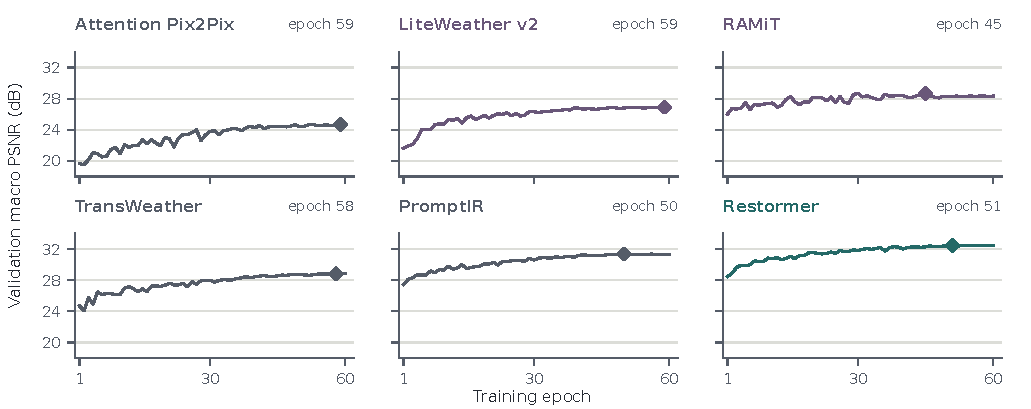
\includegraphics[width=.96\linewidth]{figures/validation_trajectories.pdf}
\captionof{figure}{Native-resolution validation PSNR across 60 epochs. Diamonds identify the best validation macro PSNR and selected epoch. Shared axes support comparison; each curve represents one training seed, with initialization sources differing across models.}
\label{fig:validation-trajectories}
\end{minipage}

Restormer selects epoch 51 at 32.45\,dB validation macro PSNR. Its compact
inference file holds 26,126,644 parameters in 104,701,712 bytes; continuation
arms start from these weights.

\subsection{Per-weather structural fidelity}
\noindent\begin{minipage}{\linewidth}
\centering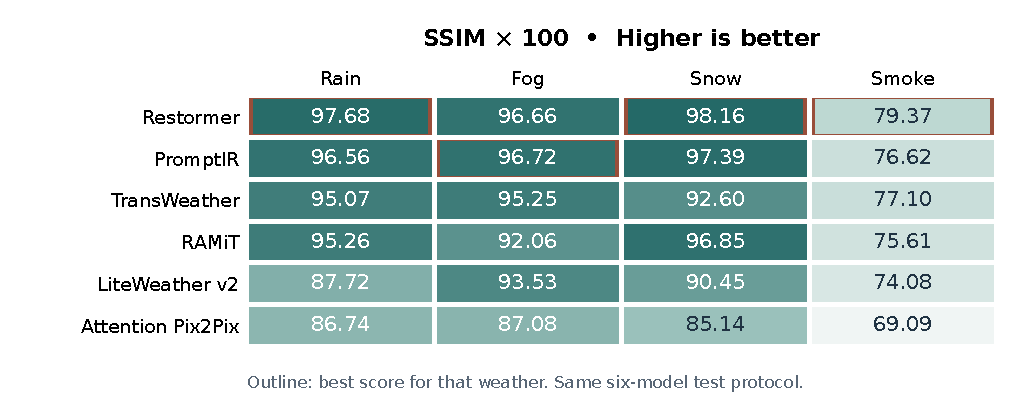
\includegraphics[width=\linewidth]{figures/weather_ssim.pdf}
\captionof{figure}{Per-weather structural similarity on 2,334 test pairs, displayed as $\mathrm{SSIM}\times100$. Outlined cells mark the best model per weather. This scaled similarity score is not detection accuracy.}
\label{fig:ssim-map}
\end{minipage}


\clearpage
\begin{multicols}{2}\raggedcolumns
The degraded-input macro is 18.62\,dB and 71.35 on the
$\mathrm{SSIM}\times100$ scale. A 2,000-resample cluster bootstrap gives
PSNR intervals of [32.00, 33.13]\,dB for Restormer and [30.81, 31.90]\,dB
for PromptIR, conditional on the trained checkpoints.

Restormer has 27 smoke PSNR regressions and 37 SSIM regressions against
raw input. Attention Pix2Pix has 179 and 341, respectively, among 342 smoke
images. The two regression sets can overlap. Display values use at most
two decimals; evidence files retain full precision.
\end{multicols}

\subsection{Preliminary rain-only baseline}
The early rain study used 784 training, 112 validation and 224 test pairs:
20 epochs, seed 42, AdamW, $128\times128$ crops and BF16 on an A100.
Validation selected epoch 15. Figure~\ref{fig:rain-progress} and
Table~\ref{tab:rain-preliminary} show mean per-image native-resolution RGB
scores for this historical checkpoint. The later four-weather benchmark
uses a distinct checkpoint and aggregation protocol.

\begin{center}\begin{minipage}{\linewidth}
\centering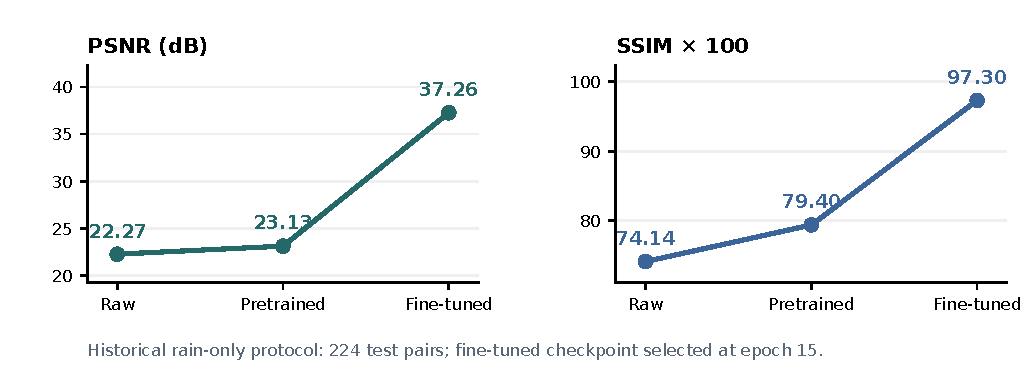
\includegraphics[width=\linewidth]{figures/historical_rain_progress.pdf}
\captionof{figure}{Measured progress in the preliminary rain-only experiment: degraded input, pretrained restoration and fine-tuned restoration. Both panels use the same 224 rain test pairs; this is separate from the six-model four-weather comparison.}
\label{fig:rain-progress}
\end{minipage}\end{center}

\begin{center}\begin{minipage}{.80\linewidth}
\centering\small
\captionof{table}{Historical rain-only benchmark; SSIM uses the $\times100$ display scale.}
\label{tab:rain-preliminary}
\begin{tabular*}{\linewidth}{@{\extracolsep{\fill}}lrr@{}}\toprule
Input or model & RGB PSNR (dB) & SSIM $\times100$\\\midrule
Raw rainy input &22.27&74.14\\
Pretrained Restormer &23.13&79.40\\
Fine-tuned Restormer, epoch 15 &37.26&97.30\\\bottomrule
\end{tabular*}
\end{minipage}\end{center}

\section{Continuation: Per-Weather Breakdown}
\label{app:joint}
The complete held-out breakdown below uses validation-selected states.
The small test differences do not change the validation replacement decision
in Section~\ref{sec:jointresults}; the epoch-51 baseline remains selected.
PSNR is in dB and SSIM is displayed on the $\times100$ scale.
\begin{center}\begin{minipage}{\linewidth}
\centering\small
\captionof{table}{Follow-up test breakdown: balanced PSNR (dB) / $\mathrm{SSIM}\times100$ for each weather. Checkpoints are selected by validation, and the original deployment model is retained before test.}
\label{tab:jointweather}
\begin{tabular}{@{}lcccc@{}}\toprule
Model / arm & Rain & Fog & Snow & Smoke\\\midrule
Original & 38.77 / 97.68 & 31.51 / 96.66 & 39.51 / 98.16 & 20.55 / 79.37\\
Continuation control & 38.70 / 97.62 & 31.79 / 96.81 & 39.57 / 98.17 & 20.75 / 79.71\\
Spatial & 38.71 / 97.63 & 31.79 / 96.82 & 39.57 / 98.17 & 20.76 / 79.71\\
Detail & 38.70 / 97.62 & 31.79 / 96.81 & 39.57 / 98.18 & 20.76 / 79.71\\
Combined & 38.70 / 97.62 & 31.80 / 96.82 & 39.57 / 98.18 & 20.76 / 79.71\\
Recipe only & 38.72 / 97.66 & 31.80 / 96.86 & 39.60 / 98.20 & 20.80 / 79.94\\
Combined + SSIM & 38.71 / 97.66 & 31.81 / 96.87 & 39.60 / 98.20 & 20.75 / 79.96\\
Combined + FFL & 38.68 / 97.59 & 31.80 / 96.82 & 39.57 / 98.17 & 20.78 / 79.66\\
Combined + recipe & 38.72 / 97.65 & 31.79 / 96.85 & 39.59 / 98.19 & 20.73 / 79.88\\
\bottomrule\end{tabular}
\end{minipage}\end{center}

\clearpage
\begingroup
\raggedbottom
\captionsetup{hypcap=false}
\section{Detection, Resolution Controls, and Nano Execution}
\label{app:hardware}

\newcommand{\AegisEvidenceColumns}[2]{%
  \noindent\begin{minipage}[t]{.477\linewidth}\vspace{0pt}#1\end{minipage}\hfill
  \begin{minipage}[t]{.477\linewidth}\vspace{0pt}#2\end{minipage}\par
}

\AegisEvidenceColumns{%
\subsection{Labelled detection protocols}
The earlier local pilot draws 72 images from 704 audited DAWN image and annotation pairs. It evaluates person, bicycle, car, motorcycle, bus, and truck. Raw, resize-only, and restored views share the same detector. Local precision and recall use each view's maximum-F1 point.

The Nano benchmark has 72 images and 541 annotations. At confidence 0.25 and IoU 0.50, unmatched predictions fall from 92 to 60 and misses rise from 271 to 431. The Nano comparison measures the complete cascade. Estimating the contribution of resampling would require a resize-only arm over the full labelled set.
}{%
\subsection{Engine identity and fixture agreement}
The original 4\,GB Nano runs L4T 32.7.3, Python 3.6.9, and TensorRT 8.2.1.8~\cite{NVIDIA_Compute,NVIDIA_TensorRT}. Its FP32 YOLOv8n passes three fixtures, with worst score error $5.51\times10^{-6}$ and box RMSE $4.63\times10^{-5}$ pixels. The epoch-51 mixed FP16/FP32 restorer passes four fixtures (Table~\ref{tab:nano-agreement}). Earlier larger builds encountered memory pressure. Section~\ref{app:quant} reports the offline export and compression screens.

\smallskip
\noindent\begin{minipage}{\linewidth}
\centering\footnotesize\renewcommand{\arraystretch}{1.12}\setlength{\tabcolsep}{3pt}
\captionof{table}{Mixed-precision $128\times128$ Nano Restormer fixture agreement. Errors use the scaled units below; $1\,\mathrm{mdB}=10^{-3}\,\mathrm{dB}$. All four fixtures pass the recorded gate.}
\label{tab:nano-agreement}
\begin{tabular}{@{}lrrr@{}}\toprule
Fixture & \shortstack{RMSE\\($\times10^{-4}$)} & \shortstack{$e_\infty$\\($\times10^{-3}$)} & \shortstack{$\Delta$PSNR\\(mdB)}\\\midrule
Fog & 1.95 & 1.72 & -1.65\\
Rain & 0.53 & 0.87 & +1.66\\
Smoke & 1.79 & 0.81 & +4.76\\
Snow & 1.35 & 1.22 & +0.09\\
\bottomrule\end{tabular}
\end{minipage}\par

}

\medskip
\noindent\begin{minipage}{\linewidth}
\centering\small\renewcommand{\arraystretch}{1.12}\setlength{\tabcolsep}{3.5pt}
\captionof{table}{Labelled DAWN results in percent. Local entries are raw / resize only / Restormer. Nano entries are YOLO only / Restormer + YOLO. Nano precision and recall use confidence 0.25 and IoU 0.50. Pooled AP is computed over 72 images.}
\label{tab:dawn-operating}
\begin{tabular}{@{}lrccccc@{}}\toprule
Subset & Images & Local AP$_{50:95}$ & Nano AP$_{50:95}$ & Nano AP$_{50}$ & Nano precision & Nano recall\\
\midrule
All & 72 & 29.97 / 29.25 / 32.86 & 29.59 / 14.50 & 44.32 / 23.06 & 74.59 / 64.71 & 49.91 / 20.33\\
Fog & 24 & 26.99 / 29.40 / 37.11 & 25.39 / 10.32 & 38.38 / 18.02 & 69.77 / 71.88 & 42.55 / 16.31\\
Rain & 24 & 38.87 / 37.07 / 37.21 & 38.91 / 29.24 & 58.74 / 39.22 & 71.76 / 65.52 & 47.24 / 19.10\\
Snow & 24 & 36.27 / 33.47 / 35.62 & 36.98 / 15.94 & 49.36 / 26.07 & 80.00 / 61.25 & 57.71 / 24.38\\
\bottomrule
\end{tabular}
\end{minipage}\par


\bigskip
\noindent\begin{minipage}{\linewidth}
\centering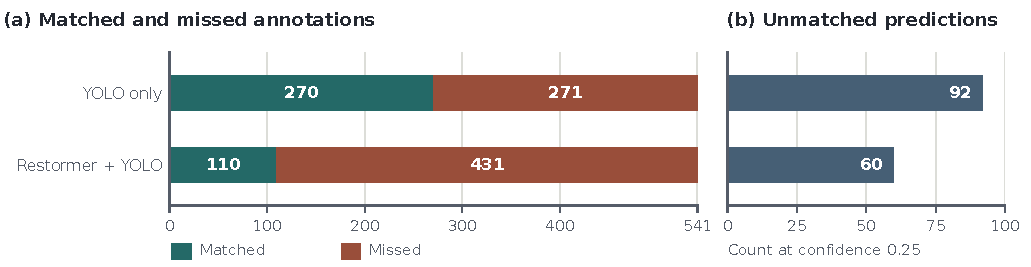
\includegraphics[width=\linewidth]{figures/nano_detection_counts.pdf}
\captionof{figure}{Object-level outcomes in labelled Nano replay. Each row in (a) accounts for all 541 annotations at confidence 0.25 and class-aware matching at IoU 0.50. The loss of matches is larger than the reduction in unmatched predictions.}
\label{fig:nano-detection-counts}
\end{minipage}

\clearpage
\subsection{Timing and power boundaries}
\AegisEvidenceColumns{%
The live application runs synthetic weather cases sequentially for about 30 seconds each. Its FPS includes capture, weather synthesis, display, and application overhead. Pipeline latency excludes weather synthesis. DAWN replay times preprocessing, transfers, inference, and NMS.
}{%
Saved-camera replay repeats 12 frames per case for at least 30 seconds. Energy integrates the board input rail, \texttt{POM\_5V\_IN}, including idle consumption. The recorded idle readings are 2.41 and 2.53\,W. These single short runs characterize the measured workloads.
}

\medskip
\noindent\begin{minipage}{\linewidth}
\centering\small\renewcommand{\arraystretch}{1.12}\setlength{\tabcolsep}{3.5pt}
\captionof{table}{Original Jetson Nano measurements. Each cell lists YOLO only / Restormer + YOLO. Live FPS includes camera and application overhead. Replay FPS excludes capture, weather synthesis, disk I/O, scoring, and output writes. Input-rail energy includes board idle consumption.}
\label{tab:nano-runtime}
\begin{tabular}{@{}llrrrr@{}}\toprule
Workload & Weather & FPS & Pipeline p50 (ms) & Input power (W) & Input J/frame\\
\midrule
Live camera & Fog & 4.72 / 0.60 & 108.2 / 1576.8 & 5.00 / 6.99 & 1.06 / 11.73\\
 & Rain & 5.02 / 0.60 & 108.4 / 1568.5 & 5.44 / 7.11 & 1.08 / 11.83\\
 & Snow & 5.28 / 0.60 & 108.4 / 1571.1 & 5.22 / 7.22 & 0.99 / 11.94\\
 & Smoke & 3.68 / 0.57 & 108.9 / 1564.8 & 4.91 / 6.91 & 1.33 / 12.21\\
\midrule
Labelled DAWN replay & Fog & 7.28 / 0.62 & 129.2 / 1596.7 & 5.71 / 7.11 & 0.78 / 11.40\\
 & Rain & 6.55 / 0.61 & 147.2 / 1617.0 & 5.38 / 7.13 & 0.82 / 11.59\\
 & Snow & 6.58 / 0.61 & 140.4 / 1619.6 & 5.34 / 6.95 & 0.81 / 11.35\\
\midrule
Saved-camera replay & Fog & 9.16 / 0.64 & 108.7 / 1560.6 & 6.17 / 7.02 & 0.67 / 10.95\\
 & Rain & 8.96 / 0.64 & 111.2 / 1562.6 & 6.11 / 7.09 & 0.68 / 11.08\\
 & Snow & 9.11 / 0.64 & 109.1 / 1556.3 & 6.18 / 7.17 & 0.68 / 11.15\\
 & Smoke & 9.11 / 0.64 & 109.1 / 1554.2 & 6.16 / 7.15 & 0.68 / 11.12\\
\bottomrule
\end{tabular}
\end{minipage}\par


\bigskip
\subsection{Saved-camera replay fidelity}
The replay compares degraded and restored frames against the same pre-mask
reference. Fog PSNR rises from 17.22 to 21.38\,dB, while SSIM falls from
90.00 to 75.67 on the $\mathrm{SSIM}\times100$ scale. Both metrics decline
in rain, snow and smoke. These pixel scores include resampling; the labelled
DAWN benchmark separately measures detection.

\begin{center}\begin{minipage}{\linewidth}
\centering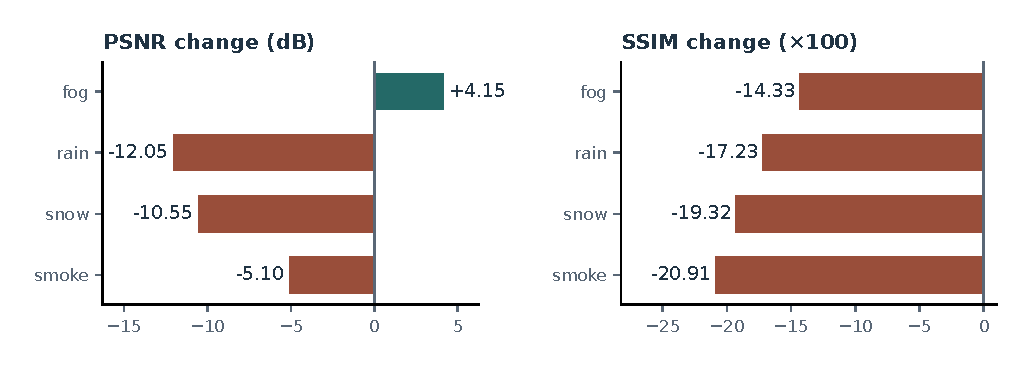
\includegraphics[width=\linewidth]{figures/camera_fidelity_scaled.pdf}
\captionof{figure}{Changes in pixel fidelity on saved-camera replay. SSIM differences use the $\times100$ display scale; neither panel measures detection accuracy.}
\label{fig:replay-fidelity}
\end{minipage}\end{center}

\clearpage
\subsection{Matched local resolution diagnostic}
\AegisEvidenceColumns{%
The diagnostic uses a $600\times315$ hazy DAWN image with two labelled vehicles, a $224\times180$ hazy RTTS photo with three labelled people, and an unlabelled $320\times240$ camera image. Fog, rain, snow, or smoke is applied once at source size (level 2, seed 43, time 0). The original views retain any pre-existing haze.

The 128 and 256 canvases preserve aspect ratio and use edge padding. Native Restormer pads to a multiple of eight and crops back. All paths return to source geometry before a $640\times640$ detector letterbox.
}{%
Six views share each degraded source, yielding 90 verified paths. Restoration uses CPU FP32. The same FP32 ONNX detector uses confidence 0.25, NMS IoU 0.7, and class-aware matching at IoU 0.50.

Across the eight added-weather variants of the labelled scenes, direct detection yields 19/0/1 (TP/FP/FN). The 256 resize-only and restored paths yield 20/2/0 and 19/4/1, respectively. Native restoration yields 19/1/1. It retains all three people under added weather and introduces one unmatched rain prediction. The same five annotations recur across conditions.
}

\medskip
\noindent\begin{minipage}{\linewidth}
\centering\small\renewcommand{\arraystretch}{1.12}\setlength{\tabcolsep}{3.5pt}
\captionof{table}{Controlled local FP32 diagnostic. Weather is applied at source resolution before branching. Labelled rows report TP/FP/FN at confidence 0.25 and IoU 0.50. Camera rows count predictions. Each source is reused across conditions.}
\label{tab:resolution-control}
\begin{tabular}{@{}lrrrrrr@{}}\toprule
Weather & Direct & 128 resize & 128 restore & 256 resize & 256 restore & Native restore\\
\midrule
\multicolumn{7}{@{}l}{\textbf{Truck/car scene, 2 labelled vehicles}}\\
Original & 2/0/0 & 1/0/1 & 1/0/1 & 2/0/0 & 2/0/0 & 2/0/0\\
Fog & 2/0/0 & 1/0/1 & 1/0/1 & 2/0/0 & 2/0/0 & 2/0/0\\
Rain & 1/0/1 & 1/1/1 & 1/0/1 & 2/0/0 & 2/0/0 & 2/0/0\\
Snow & 2/0/0 & 1/0/1 & 2/0/0 & 2/1/0 & 2/1/0 & 2/0/0\\
Smoke & 2/0/0 & 1/0/1 & 1/0/1 & 2/0/0 & 2/0/0 & 1/0/1\\
\midrule
\multicolumn{7}{@{}l}{\textbf{Small-source scene, 3 labelled people}}\\
Original & 3/0/0 & 3/0/0 & 3/0/0 & 3/0/0 & 3/1/0 & 3/1/0\\
Fog & 3/0/0 & 2/0/1 & 3/0/0 & 3/1/0 & 3/1/0 & 3/0/0\\
Rain & 3/0/0 & 3/0/0 & 3/0/0 & 3/0/0 & 3/0/0 & 3/1/0\\
Snow & 3/0/0 & 2/0/1 & 2/0/1 & 3/0/0 & 2/1/1 & 3/0/0\\
Smoke & 3/0/0 & 3/1/0 & 3/0/0 & 3/0/0 & 3/1/0 & 3/0/0\\
\midrule
\multicolumn{7}{@{}l}{\textbf{Unlabelled camera frame, prediction counts}}\\
Original & 2 & 3 & 3 & 2 & 2 & 2\\
Fog & 2 & 2 & 2 & 2 & 2 & 2\\
Rain & 2 & 3 & 3 & 2 & 2 & 2\\
Snow & 2 & 3 & 3 & 3 & 3 & 2\\
Smoke & 2 & 3 & 3 & 2 & 2 & 2\\
\bottomrule
\end{tabular}
\end{minipage}\par

\medskip

\noindent\begin{minipage}{\linewidth}
\centering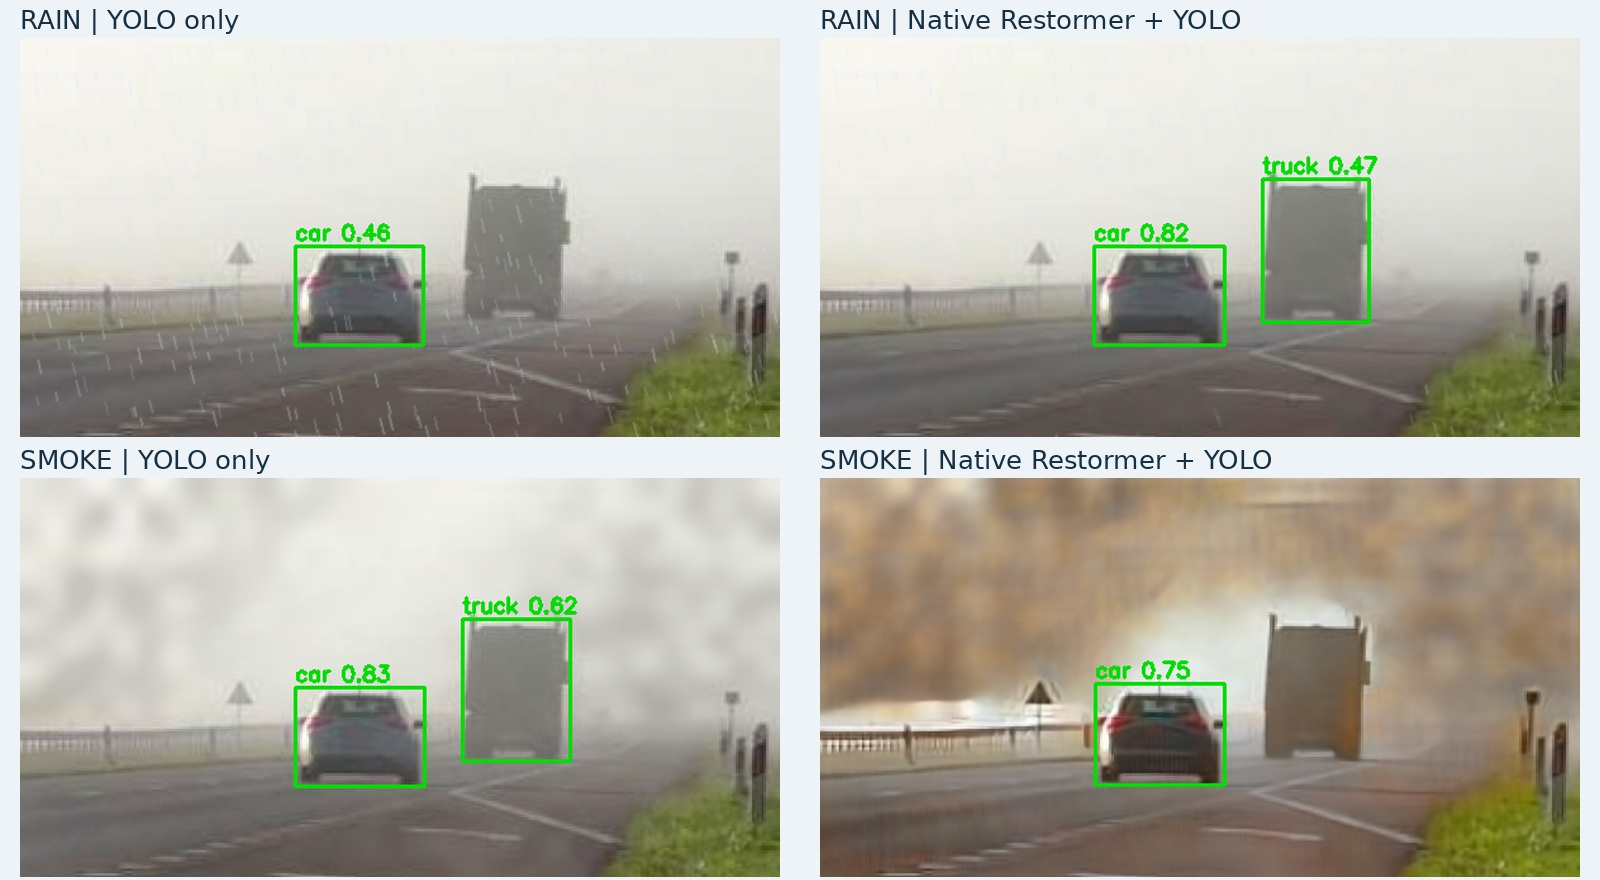
\includegraphics[width=.88\linewidth]{figures/native_detection_cases.jpg}
\captionof{figure}{Fixed-input native-resolution comparisons for the DAWN truck/car scene. The same detector finds the truck after restoration under rain and misses it after restoration under smoke. The overlays illustrate the matched counts in Table~\ref{tab:resolution-control}.}
\label{fig:native-truck}
\end{minipage}

\clearpage
\subsection{Fixed-canvas and camera controls}
\AegisEvidenceColumns{%
In the earlier fixed-$128\times128$ controls, weather is added after resizing. The people and vehicle images retain $128\times103$ and $128\times67$ pixels before padding. The truck is about $18\times26$ pixels after resizing. Resize alone removes its match in the hazy original. The small-source original retains all three people across paths.
}{%
The camera delivers $320\times240$ directly. The first of three captured frames occupies $128\times96$ before padding. Native local views yield two predictions per condition with or without restoration. The camera views lack ground-truth annotations.
}

\medskip
\noindent\begin{minipage}{\linewidth}
\centering
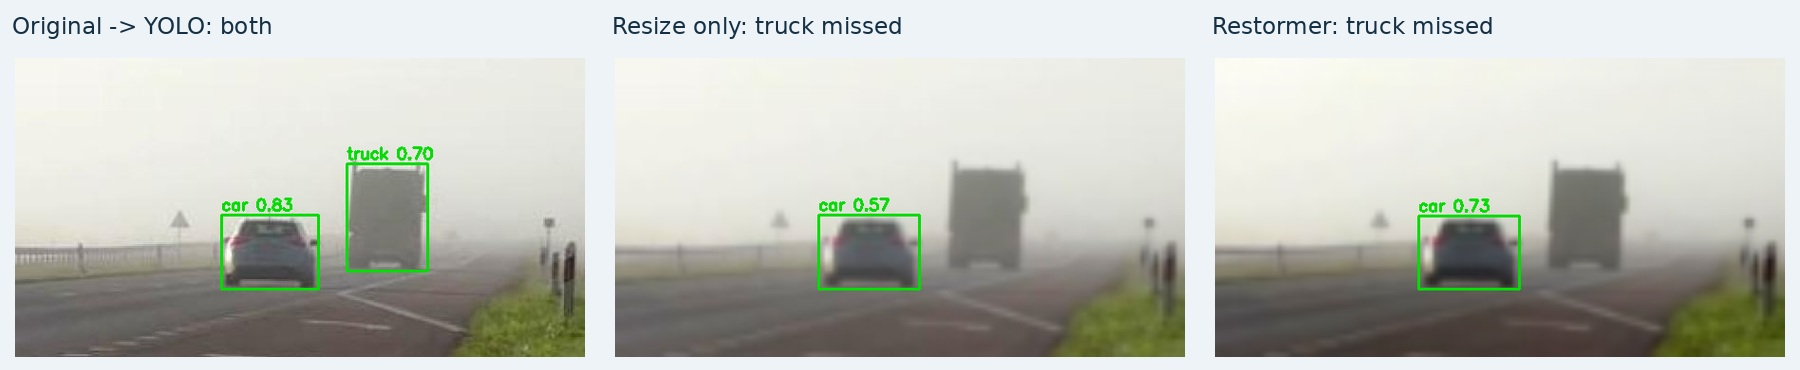
\includegraphics[width=.84\linewidth]{figures/truck_128_control.jpg}\par\smallskip
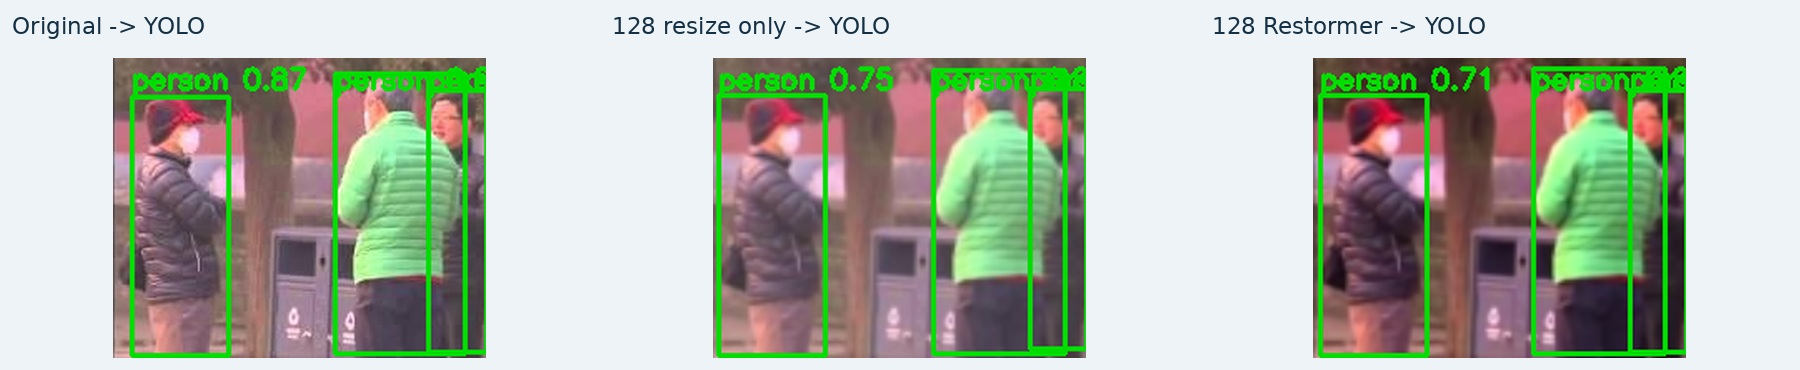
\includegraphics[width=.84\linewidth]{figures/small_source_128_control.jpg}
\captionof{figure}{Fixed-canvas controls without added synthetic weather. The truck is detected at source size and missed in both 128 paths. All three paths detect the annotated people in the small RTTS source. Images are enlarged from saved outputs.}
\label{fig:fixed-canvas}
\end{minipage}

\medskip
\noindent\begin{minipage}{\linewidth}
\centering\small\renewcommand{\arraystretch}{1.12}\setlength{\tabcolsep}{3.5pt}
\captionof{table}{Fixed-$128\times128$ Nano diagnostics. Synthetic weather is added after resizing. Labelled rows show TP/FP/FN. Camera entries count predictions. Timing is median pipeline latency over repeated calls on each input.}
\label{tab:fixed-diagnostics}
\begin{tabular}{@{}llrrr@{}}\toprule
Source & Weather & Resize + YOLO & Restormer + YOLO & Median ms, resize / restored\\
\midrule
RTTS people & Original & 3/0/0 & 3/0/0 & 117.1 / 1554.7\\
 & Rain & 2/0/1 & 2/1/1 & 115.7 / 1560.3\\
 & Snow & 2/0/1 & 2/0/1 & 114.5 / 1560.6\\
 & Smoke & 3/1/0 & 3/0/0 & 116.9 / 1561.8\\
\midrule
DAWN truck/car & Original & 1/0/1 & 1/0/1 & 119.1 / 1563.6\\
 & Rain & 0/1/2 & 1/0/1 & 120.3 / 1562.7\\
 & Snow & 1/0/1 & 1/0/1 & 122.4 / 1566.8\\
 & Smoke & 1/0/1 & 1/0/1 & 120.5 / 1566.8\\
\midrule
320 × 240 camera & Original & 3 & 3 & 115.4 / 1564.7\\
 & Rain & 4 & 2 & 118.7 / 1563.0\\
 & Snow & 4 & 4 & 119.0 / 1562.2\\
 & Smoke & 3 & 2 & 116.8 / 1565.0\\
\bottomrule
\end{tabular}
\end{minipage}\par


\medskip
\noindent\begin{minipage}{\linewidth}
\centering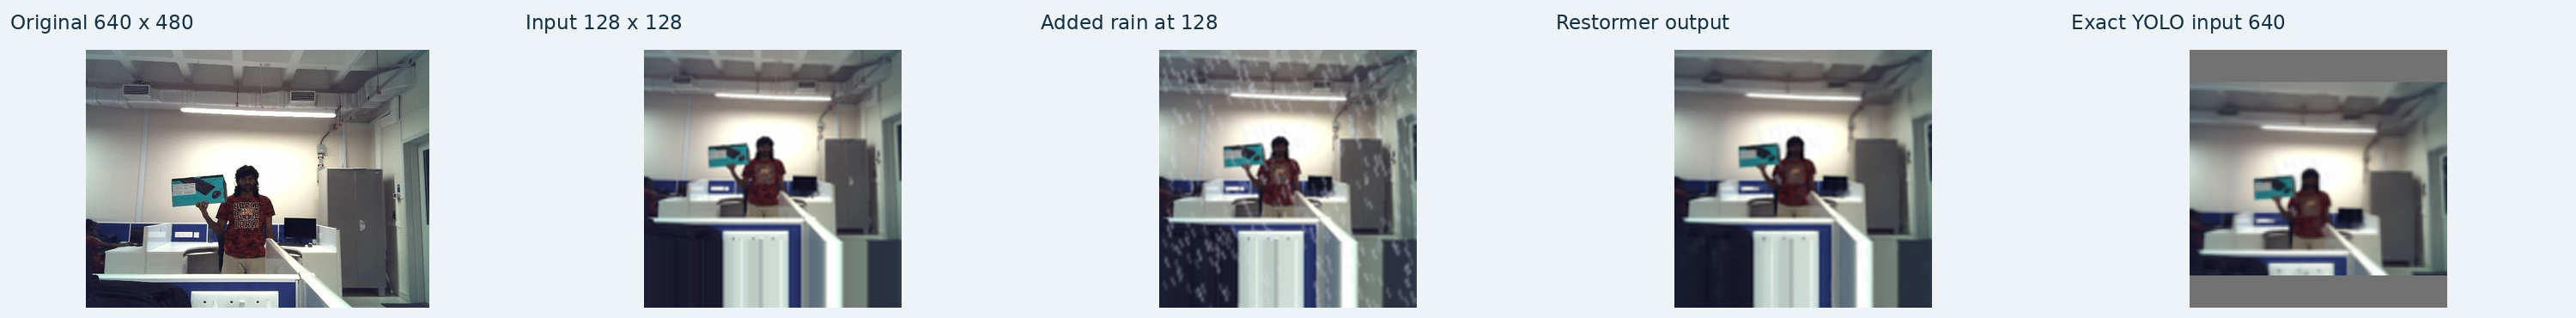
\includegraphics[width=.94\linewidth]{figures/camera_path_example.jpg}
\captionof{figure}{A separate saved $640\times480$ camera frame. The frame occupies $128\times96$ image pixels before padding. Synthetic rain is applied on the canvas. The restored result maps back to source geometry for detection.}
\label{fig:camera-path}
\end{minipage}
\clearpage
\endgroup

\clearpage
\section{Reproducibility and Evidence Map}
\label{app:repro}
\subsection{Records needed to reproduce the report}
The report uses saved experiment outputs; its preparation did not retrain
models, rerun full-set inference, or repeat board measurements. The manuscript
evidence verifier checks 35 file hashes, split counts and groups, six-model
native test aggregates, checkpoint identities, continuation results and the
local detection table. The later Nano source index supplies separate hashes
for the November 11 summaries and resolution controls.

\begin{table}[htbp]
\centering\small
\caption{Repository evidence map. Paths are relative to the project root.
The accompanying report audit records input hashes and figure/table use.}
\label{tab:evidence-map}
\begin{tabularx}{\textwidth}{@{}p{.22\textwidth}Y@{}}
\toprule Report component & Primary records and implementation\\\midrule
Frozen paired split & \path{data/manifests/weather_v3/active.csv}; \path{docs/manuscript/evidence/data_protocol.json}; \path{src/aegis_perception/data/sampling.py}\\
Model identity and quality & \path{docs/manuscript/evidence/six_models.json}; \path{docs/manuscript/tables/six_models.csv}; \path{artifacts/models/index.json}\\
Aggregation and uncertainty & \path{src/aegis_perception/evaluation.py}; \path{docs/manuscript/evidence/per_image_restoration.csv.gz}\\
Restorer implementation & \path{src/aegis_perception/models/restormer.py}; \path{src/aegis_perception/models/liteweatherformer_v2.py}; \path{configs/restoration/official_v1/sources.json}\\
Continuation and calibration & \path{docs/manuscript/evidence/joint_experiments.json}; \path{configs/restoration/joint_v3/}; \path{research/restormer_joint_v3/}\\
Local DAWN pilot & \path{docs/manuscript/tables/detection_pilot72.csv}; \path{scripts/deployment/edge_dawn.py}\\
Compression screens & \path{docs/manuscript/evidence/custom_quantization_screen.json}; \path{docs/manuscript/tables/pruning_screen.csv}\\
Nano accuracy and runtime & \path{artifacts/edge_v1/nano_20261111/consolidated_report_v2/sources/}; \path{scripts/weather_testing/score_nano_real.py}\\
Matched resolution & \path{artifacts/edge_v1/nano_20261111/resolution_accuracy_v1/}; source and detector-input verification for 90 paths\\
\bottomrule
\end{tabularx}
\end{table}

\subsection{Checkpoint and metric identity}
The selected six-model Restormer is epoch 51. Its compact inference file has
SHA-256
\begin{quote}\small\ttfamily
5268af32c161413502a8978a839b3111\\
52a1dd2bf093ade137e07d58166a8555
\end{quote}
The original deraining initialization, historical epoch-15 rain model,
earlier four-weather run and continuation arms must not be substituted for
this checkpoint. The same rule applies to model version: the evaluated
LiteWeather v2 is not the retained legacy convolutional implementation.

Image-based PSNR and SSIM use clean targets. Export agreement compares two
model outputs. AP uses labelled objects and explicitly configured confidence,
matching and suppression rules. Runtime uses the timing boundary of its
workload. These measures answer different questions even when they share
an input image or checkpoint.

\subsection{Interpretation of dated evidence}
The 5 November deployment notes describe a period before the later complete
Nano measurements. The 11 November accuracy and telemetry records establish
that the stated replay and live workloads ran; they do not establish sustained
operational acceptance. Historical documents are preserved with their original
status. Present-day report statements use the relevant dated record instead
of merging planned Orin performance with measured original-Nano performance.

\subsection{Result precision and reuse}
Numerical tables and charts use at most two decimals for readability. Small
agreement errors are displayed in scaled units, and SSIM is shown as
$\mathrm{SSIM}\times100$ where labelled. Rounding affects presentation only;
checkpoint selection and acceptance decisions use the saved full-precision
records. Independent reproduction of the experiments requires the original
data, weights, configurations and target hardware.

\end{document}
